\PassOptionsToPackage{utf8}{inputenc}
\documentclass{bioinfo}

\usepackage{makecell}

\usepackage{floatrow}

\usepackage{comment}

\usepackage{siunitx}

% singlelinecheck=false puts subcaptions on the left
\usepackage[singlelinecheck=false]{subcaption}

\usepackage{amsthm}
\theoremstyle{definition}
\newtheorem{definition}{Definition}[section]
\newtheorem{theorem}{Theorem}[section]
\newtheorem{corollary}{Corollary}[theorem]
\newtheorem{lemma}[theorem]{Lemma}

\usepackage{amsfonts}
\usepackage{booktabs}

\usepackage{algorithm2e}
\usepackage[usenames,dvipsnames]{xcolor}
\SetAlgoLined
\usepackage{bm}

% we squeeze our figures even more together
\captionsetup{belowskip=-2pt}

\SetAlgoLined
\SetKwProg{MyStruct}{Struct}{ contains}{end}

\newcommand{\vocab}{\textbf}
\newcommand{\red}[1]{{\textcolor{Red}{#1}}}
\newcommand{\FIXME}[1]{\red{[FIXME: #1]}}

\usepackage{orcidlink}
\hypersetup{hidelinks}
\usepackage{appendix}
\newcommand{\description}{}
\usepackage[inline]{enumitem}

% table stuff
\usepackage{amsfonts}
\usepackage{booktabs}
\usepackage{siunitx}
\newcommand{\ra}[1]{\renewcommand{\arraystretch}{#1}}
\usepackage{float}
\usepackage{hyperref}
\floatstyle{plaintop}
\restylefloat{table}

% supplement stuff
\newcommand{\beginsupplement}{%
	\setcounter{table}{0}
	\renewcommand{\thetable}{S\arabic{table}}%
	\setcounter{figure}{0}
	\renewcommand{\thefigure}{S\arabic{figure}}%
}

\def\labelitemi{--}

\copyrightyear{2023} \pubyear{XXXX}

\access{Advance Access Publication Date: Day Month Year}
\appnotes{Genome Analysis}

\begin{document}
    \firstpage{1}

    \subtitle{Genome Analysis}

    \title[Pangenome graph layout by Path-Guided Stochastic Gradient Descent]{Pangenome graph layout by Path-Guided Stochastic Gradient Descent}
    %\title[Genome-guided pangenome graph layouts via Stochastic Gradient Descent]{Genome-guided pangenome graph layouts via Stochastic Gradient Descent}
	%\title[Sequence-guided pangenome graph layouts via Stochastic Gradient Descent]{Sequence-guided pangenome graph layouts via Stochastic Gradient Descent}
    %\title[Genome-guided pangenome graph layouts]{Genome-guided pangenome graph layouts}
	%\title[Sequence-guided pangenome graph layouts]{Sequence-guided pangenome graph layouts}
    
	\author[Heumos, Guarracino \textit{et~al}.]{
        Simon~Heumos\,$^{\orcidlink{0000-0003-3326-817X}1,2,\dagger}$,
        Andrea~Guarracino\,$^{\orcidlink{0000-0001-9744-131X}3,4,\dagger}$,
        Jan-Niklas Manuel Schmelzle\,$^{\orcidlink{0000-0001-8566-4049}5,6}$,
        Jiajie Li\,$^{\orcidlink{0000-0002-6775-2843}6}$,
        Zhiru Zhang\,$^{\orcidlink{0000-0002-0778-0308}6}$,
        Jörg Hagmann\,${\orcidlink{0000-0002-7232-3103}^7}$,
        Sven Nahnsen\,$^{\orcidlink{0000-0002-4375-0691}1,2}$,
        Pjotr Prins\,$^{\orcidlink{0000-0002-8021-9162}3}$,
        Erik~Garrison\,$^{\orcidlink{0000-0003-3821-631X}\text{\sfb 3},*}$
    }

    \address{
        $^1$Quantitative Biology Center (QBiC), University of Tübingen, Tübingen 72076, Germany \\
        $^2$Biomedical Data Science, Department of Computer Science, University of Tübingen, Tübingen 72076, Germany \\
        $^3$Department of Genetics, Genomics and Informatics, University of Tennessee Health Science Center, Memphis, TN 38163, USA \\
        $^4$Genomics Research Centre, Human Technopole, Milan 20157, Italy \\
        $^5$Department of Computer Engineering, School of Computation, Information and Technology (CIT), Technical University of Munich, Munich 80333, Germany \\
        $^6$School of Electrical and Computer Engineering, Cornell University, Ithaca, NY 14853, USA \\
        $^7$Computomics GmbH, Eisenbahnstr. 1, 72072 Tübingen, Germany \\
    }

    \corresp{
        $^\ast$To whom correspondence should be addressed. \\
        $^{\dagger}$The authors wish it to be known that, in their opinion, the first two authors should be regarded as Joint First Authors.\
    }

    \history{Received on XXXXX; revised on XXXXX; accepted on XXXXX}

    \editor{Associate Editor: XXXXXXX}

	\abstract{
	\textbf{Motivation:}
	The increasing availability of complete genomes demands for models to study genomic variability within entire populations.
	Pangenome graphs capture the full genetic diversity between multiple genomes, but their layouts may exhibit complex structures due to common, nonlinear patterns of genome variation and evolution.
	These structures hamper downstream analyses, visualization, and interpretation. \\
	\textbf{Results:}
	In response, we introduce a novel graph layout algorithm: the Path-Guided Stochastic Gradient Descent (PG-SGD).
	PG-SGD uses the genomes, represented in the pangenome graph as paths, to move pairs of nodes in parallel applying a modified HOGWILD! strategy.
	We show that our implementation efficiently computes the layout of gigabase-scale pangenome graphs, unveiling their biological features. \\
	\textbf{Availability:}
	We integrated PG-SGD in \textit{ODGI} which is released as free software under the MIT open source license.
	Source code is available at \url{https://github.com/pangenome/odgi}. \\% and documentation at \url{https://odgi.readthedocs.io/en/latest/rst/tutorials/sort_layout.html}. \\
	\textbf{Contact:} \href{egarris5@uthsc.edu}{egarris5@uthsc.edu} \\
	\textbf{Supplementary information:} Supplementary data are available at \textit{Bioinformatics} online.
	}
	
	\maketitle

	\section{Introduction}
	Reference genomes are widely used in genetics, serving as a foundation for a variety of analyses, including gene annotation, read mapping, and variant detection \citep{Singh2022}.
	However, this linear model is becoming obsolete given the accessibility to hundreds or even thousands of high-quality genomes.
	A single genome can not fully represent the genetic diversity of any species, resulting in reference bias \citep{Ballouz2019}.
	In contrast, a pangenome models the entire set of genomic elements of a given population \citep{Tettelin_2008,cpang2018,Eizenga_2020, Sherman_2020}.
	Pangenomes can be represented as a sequence graph incorporating sequences as nodes and their relationships as edges \citep{Hein1989}.
	%These nodes are shared for identical sequences, such as homologs, paralogs, and orthologs.
	In the variation graph model \citep{Garrison:2018}, genomes are encoded as paths traversing the nodes in the graph.
	%A bidirected graph can even contain both strands of DNA as paths. \\
	
	A pangenome graph layout is the arrangement of nodes and edges in an \textit{N}-dimensional space to produce a human-readable visualization of genetic variation between multiple genomes.
	Layout algorithms aim to find optimal node coordinates in order to minimize overlapping nodes or edges, reduce edge crossings, and promote an intuitive graph understanding.
	One popular approach is force-directed graph drawing \citep{cheong_force-directed_2022} which produces aesthetic layouts.
	This is prone to get stuck in local minima, but stochastic gradient descent (SGD) implementations alleviate such a problem \citep{Zheng2019}.
	SGD uses the gradient of its individual terms to approximate the gradient of a sum of functions.
	%Specifically, in pangenome graphs we move a single pair of nodes at a time.
	
	Typically, force-directed layouts are hard to compute \citep{wang_research_2014}, but the lock-free HOGWILD! method offers a highly parallelizable and thus scalable SGD approach that can be applied when the optimization problem is sparse \citep{Recht2011}.
	
	In practice, multidimensional scaling (MDS) is applied to minimize the difference between the visual distance and theoretical graph distance.
	This can be accomplished by using pairwise node distances to minimize an energy function.
	Since pangenome graphs represent genomes as paths in the graph, a reasonable distance metric would be the nucleotide distance between a pair of nodes traversed by the same path.
	
	Here, we present a new pangenome graph layout algorithm which applies a path-guided stochastic gradient descent (PG-SGD) to move pairs of nodes in parallel with a modified HOGWILD! strategy.
	The algorithm computes the pangenome graph layout that best reflects the nucleotide sequences in the graph.
	To our knowledge, no algorithm takes into account such biological information to compute the graph layouts.
	PG-SGD can be extended in any number of dimensions.
	In the ODGI toolkit \citep{Guarracino2022}, we provide implementations for 1-dimensional (1D) and 2-dimensional (2D) layouts.

	\section{Algorithm}

	While PG-SGD is inspired by \cite{Zheng2019}, we designed the algorithm to work on the variation graph model (Definition \ref{def:vg}).
	
	\begin{definition}
		\label{def:vg}
		Variation graphs are a mathematical formalism to represent pangenome graphs \citep{Garrison_2019_thesis}.
		In the variation graph $\mathcal{G} = (\mathcal{V}, \mathcal{E}, \mathcal{P})$, nodes (or vertices) $\mathcal{V} = v_1\ldots v_{|\mathcal{V}|}$ contain nucleotide sequences.
		Each node $v_i$ has a unique identifier $i$ and an implicit reverse complement $\bar{v_i}$.
		The node strand $o$ represents the node orientation.
		Edges $\mathcal{E} = e_1\ldots e_{|\mathcal{E}|}$ connect ordered pairs of node strands ($e_i = ( o_a, o_b )$), defining the graph topology.
		Paths $\mathcal{P} = p_1\ldots p_{|\mathcal{P}|}$ are series of connected steps $s_i$ that refer to node strands in the graph ($p_i = s_1 \ldots s_{|p_i|}$); the paths represent the genomes embedded in the graph.
	\end{definition}
	
	We report PG-SGD's pseudocode in Algorithm~\ref{alg:pg_sgd} and its schematic in Figure~\ref{fig:sketches}.
	In brief, the algorithm moves one pair of nodes $( v_i, v_j )$ at a time, minimizing the difference between the layout distance $ld_{ij}$ of the two nodes and the nucleotide distance $nd_{ij}$ of the same nodes as calculated along a path that traverses them.
	In the 2D layouts, nodes have two ends.
	When moving a pair of nodes, we actually move one end of each node.
	$v_i$ is the node associated with the step $s_i$ sampled uniformly from all the steps in $\mathcal{P}$.
	$v_j$ is the node associated with the step $s_j$ sampled from the same path of $s_i$ by drawing a Zipfian distribution \citep{Zipf1932}.
	The difference between $nd_{ij}$ and $ld_{ij}$ guides the update of the node coordinates in the layout.
	The magnitude $r$ of the update depends on the learning rate $\mu$.
	The number of iterations steers the annealing step size $\eta$ which determines the learning rate $\mu$.
	%A key property of pangenome graph layouts is that their nodes can be arranged so that most edges go between nodes that are close together in the node order \citep{Guarracino2022}.
	A large $\eta$ in the first iterations leads to a globally linear (in 1D) or planar (in 2D) layout.
	By decreasing $\eta$, the layout adjustments become more localized, ensuring that the nodes are positioned to best reflect the nucleotide distances in the paths (i.e., in the genomes).

	\SetKwProg{for}{for}{:}{end}
\SetKwProg{pgsgd}{PG-SGD}{:}{end}
\SetKwProg{each}{for each}{:}{end}
\SetKwProg{IF}{if}{:}{end}

\SetKwFunction{PathIndex}{PathIndex}
\SetKwFunction{LayoutInitialization}{LayoutInitialization}
\SetKwFunction{InitZipf}{InitZipf}
\SetKwFunction{Unif}{Unif}
\SetKwFunction{Zipf}{Zipf}
\SetKwFunction{StepCount}{StepCount}
\SetKwFunction{Path}{Path}
\SetKwFunction{StepPos}{StepPos}

\begin{algorithm}
	\pgsgd{\textbf{(}$\mathcal{G}$\textbf{)}}{
		\textbf{input:} variation graph $\mathcal{G} = (\mathcal{V}, \mathcal{E}, \mathcal{P})$ \\
		%https://tex.stackexchange.com/questions/22643/how-to-write-letters-in-bold-in-the-math-mode
		\textbf{output:} $N$-dimensional layout $\mathcal{L}$ with $|\mathcal{V}|$ nodes \\
		$\mathcal{XP}$ $\gets \PathIndex(\mathcal{G})$ \tcp{for path position lookup} 
		%\boldsymbol{$Z$} $\gets ZipfZetas(G,P)$ \\ %@Andrea is this correct like this?
		$\mathcal{L}$ $\gets \LayoutInitialization(\mathcal{V}, N)$ \\ %\tcp{random or deterministic} 
		$\mathcal{Z} \gets \InitZipf(\mathcal{G},\mathcal{XP})$ \tcp{Zipfian distribution}
		% atomic positions initialization?
		% TODO for simplicity reasons I would only describe the 2D one here
		\for{$\eta$ $in$ $annealing$ $schedule$}{ %our "schedule" actually is the number paths.... we should specify this I would say
			\each{$planned$ $term$ $update$} { % I think we can remove i<j, because we don't care about that
				$s_i \gets \Unif(\mathcal{XP})$ \tcp{uniform sampling of a step from $\mathcal{P}$}
				$p \gets \Path(s_i,\mathcal{XP})$ \tcp{path of $s_i$}
				\uIf{$(cooling$ $||$ $flip)$} {
					$s_j \gets \Unif(\StepCount(p, \mathcal{XP}))$ \tcp{uniform sampling of a step from $p$}
				} \Else {
					$s_j \gets \Zipf(p)$ \tcp{Zipfian sampling of a step from $p$}
				}
				$p_i \gets \StepPos(s_i)$ \tcp{nuc. position}
				$p_j \gets \StepPos(s_j)$ \tcp{nuc. position}
				$nd_{ij} \gets ||p_i - p_j||$ \tcp{nuc. distance} %mag is nx
				$ld_{ij} \gets ||l_{i} - l_j||$ \tcp{layout distance}
				$w_{ij} \gets \frac{1.0}{nd_{ij}}$ \tcp{term weight} 
				$\mu \gets w_{ij}\eta$ \tcp{learning rate}  % current learning rate is given by term weight and step size
				\IF{$\mu>1$} {
				$\mu \gets 1$
				}
				$\delta \gets \mu \cdot \frac{ld -nd_{ij}}{2}$ \tcp{the actual delta}
				\uIf{$\delta <= 0$} {
					$STOP$ \tcp{we can't optimize more}
				}
				% TODO stop early?
				% TODO potentially store new delta max?
				$r \gets \delta - ld_{ij}$ \tcp{size of the update}
				$l_i \gets l_i - r\cdot ld_{ij}$ \tcp{update $v_i$ coordinates}
				$l_j \gets l_j - r\cdot ld_{ij}$ \tcp{update $v_j$ coordinates}
			}
		}
	}
	\caption{Pseudocode of PG-SGD.}
	\label{alg:pg_sgd}
\end{algorithm}

	%In standard SGD layout algorithms, the problem space is given by pairwise node comparisons.
	%In PG-SGD, the problem space is given by the pairwise path step comparisons.
	%The number of path steps in large variation graphs can be several orders of magnitude higher than the number of nodes.
	%Therefore, the number of term updates in PG-SGD is bound to the number of path steps in the graph.
	%Should the delta of $nd_{ij}$ and $ld_{ij}$ become 0 before the annealing schedule is finished, the algorithm stops.

	Originating from empirical inspection of word frequency tables, Zipf's law states that a word with rank $n$ occurs $1/n$ times as the most frequent one.
    This law is modeled by the Zipf distribution.%, whose rank-frequency distribution is related to the inverse power law. % repetitive
	Sampling $s_j$ from a Zipf distribution fixed in the $s_i$'s path position space increases the possibility to draw a nucleotide position close to $s_i$.
	So there is a high chance to use small nucleotide distances $nd_{ij}$ to refine the layout of nodes comprising a few base pairs.
    The Zipf distribution is also long-tailed, with many occurrences of low frequency events.
	However, extremely long-range correlations might not be captured sufficiently, resulting in collapsed layouts for structures that are otherwise linear.
    To provide balance between global and local layout updates, in half of the updates ($flip$ flag in Algorithm~\ref{alg:pg_sgd}), the $s_j$ is sampled uniformly instead from a Zipf distribution, with uniform sampling being more favorable for global updates.
	Furthermore, to enhance local linearity (in 1D) or planarity (in 2D) of the graph layout, a \textit{cooling} phase skews the Zipfian distribution after half of iterations have been completed.
	This increases the likelihood of sampling smaller nucleotide distances for the layout updates.

	\begin{figure*}[!htb]
	\centering
		%\hline
		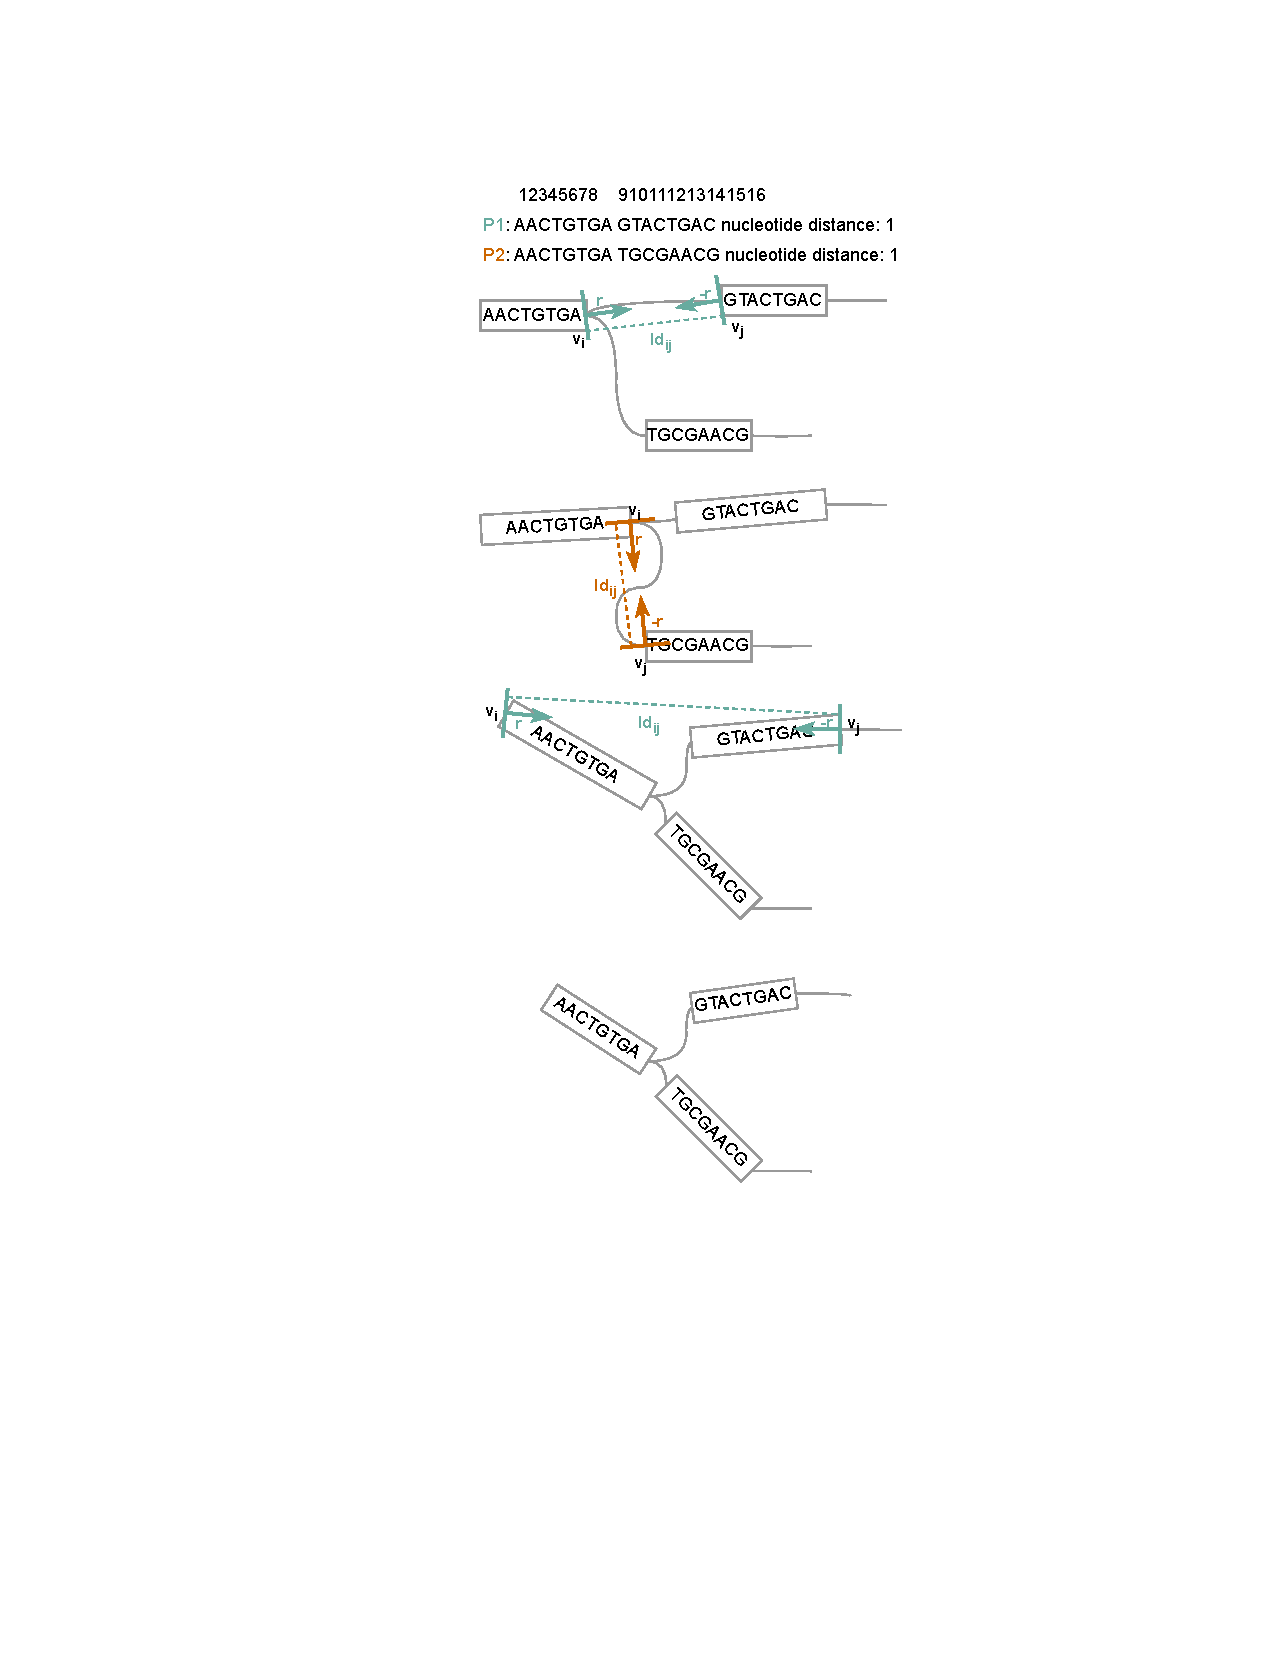
\includegraphics[width=\linewidth, trim=0cm 8cm 0cm 0cm, clip]{fig/sketches/PG-SGD.drawio.pdf}
	\caption{
		2D PG-SGD update operation sketches. \\
		\FIXME{ADD CAPTION.} \\ 
		\FIXME{PROVIDE SEVERAL NICE FIGURES SO WE CAN REARRANGE STUFF INTO SUBFIGURES.}
	}
	\label{fig:sketches}
\end{figure*}

	\section{Implementation}
	
	We implemented PG-SGD in ODGI \citep{Guarracino2022}: the 1D version can be found in \textit{odgi sort} and the 2D version in \textit{odgi layout}. % which serves as an interface to graphs in the GFA (\url{https://github.com/GFA-spec/GFA-spec}) format.
	To efficiently retrieve path nucleotide positions, we implemented a path index.
	This index is a strict subset of the XG index~\citep{Garrison:2018} where we avoid to use succinct SDSL data structures \citep{Gog2014}.
	Instead, we rely on bit-compressed integer vectors, enabling efficient retrieval of path nucleotide positions to quickly compute nucleotide distances without having to store all pairwise distances between nodes in memory.
	This approach ensures to scale on large pangenome graphs representing thousands of whole genomes.

	Graph layout initialization can significantly influence the quality of the final layout.
	In the 1D implementation, by default, nodes are placed in the same order as they appear in the input graph, although we also provide support for random layout initialization.
	In 2D, we offer several layout initialization techniques.
	One approach places nodes in the first layout dimension according to their order in the input graph, adding either uniform or Gaussian noise in the second dimension.
	Another strategy arranges nodes along a Hilbert curve, an approach that often favors the creation of planar final layouts.
	We also support fixing node positions to keep nodes in the same order as they are in a selected path, such as a reference genome.
	This feature allows us to build reference-focused graph layouts (Figure~\ref{fig:1d_fig4}).

	Our implementation is multithreaded and uses shared memory for storing the layout in a vector, according to the HOGWILD! strategy \citep{Recht2011}.
	Threads perform layout updates without any locking for additional speed up.
	This approach is feasible since pangenome graphs are typically sparse \citep{Guarracino2022}, with low average node degree.
	As a result, the updates only modify small parts of the entire layout.
	While the HOGWILD! SGD algorithm writes the layout updates to a shared non-atomic double vector, PG-SGD stores node coordinates in a vector of atomic doubles.
	This vector prevents any potential memory overwrites.
	Our tests revealed basically no performance loss with respect to the non-atomic counterpart.

	%Fig. 1: Describe how our approach works, especially a single update operation (Fig. \ref{fig:sketches}). Explanation of 1D graph updating in Figures \ref{fig:1d_before_update}-\ref{fig:1d_after_update}. Explanation of 2D graph updating in Figures \ref{fig:2d_before_update}-\ref{fig:2d_after_update}. Zipf distribution.
	%\begin{figure*}[!htb]
	\centering
		%\hline
		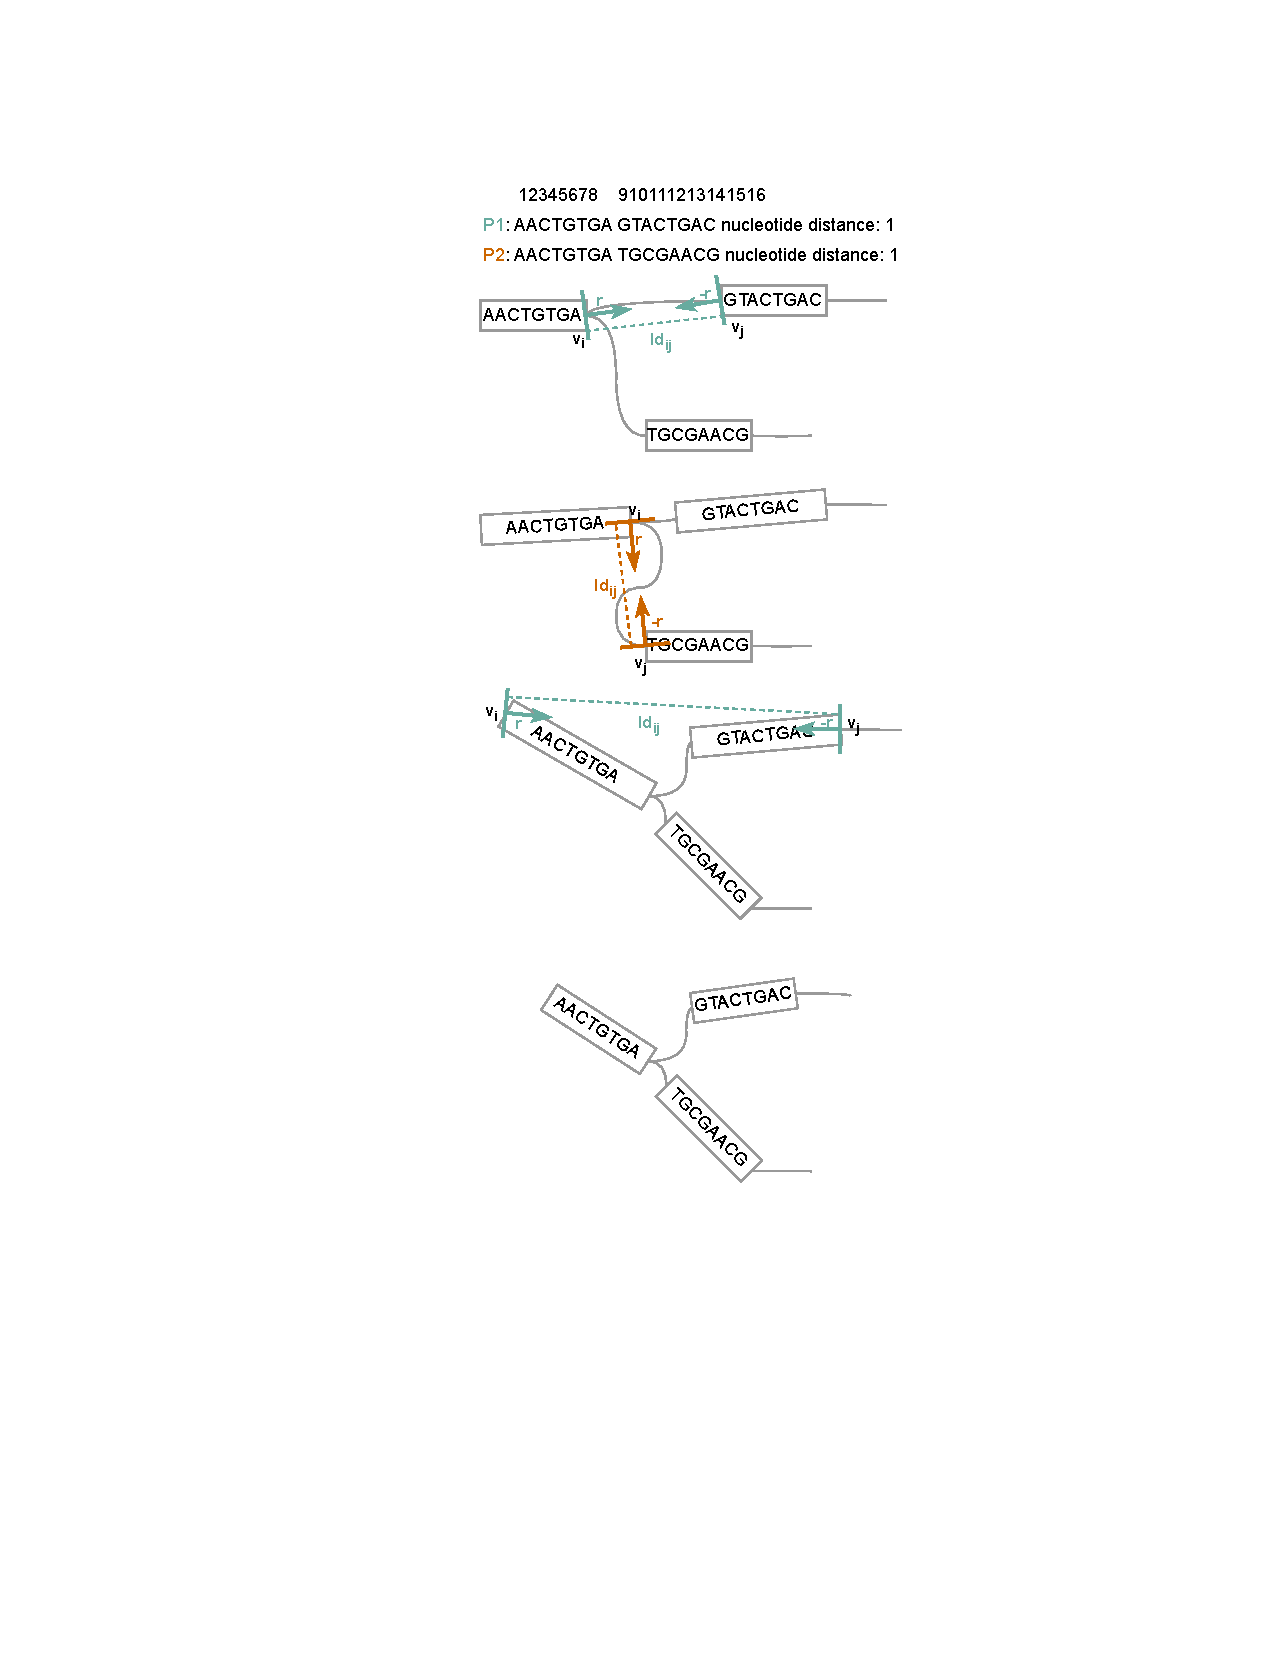
\includegraphics[width=\linewidth, trim=0cm 8cm 0cm 0cm, clip]{fig/sketches/PG-SGD.drawio.pdf}
	\caption{
		2D PG-SGD update operation sketches. \\
		\FIXME{ADD CAPTION.} \\ 
		\FIXME{PROVIDE SEVERAL NICE FIGURES SO WE CAN REARRANGE STUFF INTO SUBFIGURES.}
	}
	\label{fig:sketches}
\end{figure*}

    \section{Results}
    \label{sec:results}

    \subsection{Performance}
	We apply the 2D PG-SGD to the human pangenome \citep{Liao2023} from the Human Pangenome Reference Consortium (HPRC) to show the scalability of the algorithm.	
	Experiments were conducted on a cluster with 24 \texttt{Regular} nodes (32 cores / 64 threads with two AMD EPYC 7343 processors with 512 GB RAM) and 4 \texttt{HighMem} nodes (64 cores / 128 threads with two AMD EPYC 7513 processors with 2048 GB RAM).
	We downloaded pangenome graphs for each autosome (24 in total) and for the mitochondrial DNA.
	Each graph represents 90 whole human haplotypes: 44 diploid individuals plus the GRCh38 \citep{Schneider2017} and CHM13 \citep{Nurk_2021} haploid human references (see Supplementary Table~\ref{tab:layout} for graph statistics).
	When applied to these pangenome graphs using one \texttt{Regular} node for each calculation, 2D PG-SGD obtains the graph layouts in 50 minutes on average, with the highest run time observed being chromosome 16 (Supplementary Table~\ref{tab:layout}).
	This is expected since chromosome 16 has one of the highest levels of segmentally duplicated sequence among the human autosomes \citep{Martin2004}.
	Repetitive sequences lead to graph nodes with a very high number of path traversals, which are computationally expensive to work with \citep{Guarracino2022}.
	Memory consumption is 29.66 GB of RAM on average, with the memory peak again occurring with chromosome 16, due to the path index building phase.
	Given its scalability, we even applied PG-SGD to the full graph with all chromosomes together using a \texttt{HighMem} node (Supplementary Table~\ref{tab:layout}). 
	%A 2D layout was calculated in under one day.
	\textit{BandageNG} (\url{https://github.com/asl/BandageNG}, last accessed Jul 2023), the current state-of-the-art for graph visualization, was not able to produce a layout within 7 days, hitting the wall clock time limit of the cluster.
	On average, PG-SGD is $\sim$8X faster than BandageNG while using $\sim$2X less memory.
	% avg time bng 388 min, avg gb ng 66.84

    \subsection{Pangenome graphs layouts reveal biology features}
	Graph visualization is essential for understanding pangenome graphs and the genome variation they represent. 
	We show how 2D PG-SGD allows us gaining insight into biological data by looking at the graph layout structure. 
	%To demonstrate this, we provide various 2D PG-SGD layouts in Figure~\ref{fig:2d_layouts}.
			\begin{figure*}[!htb]
	\centering
	\begin{subfigure}{1.0\textwidth}
		\centering
		\caption{}
		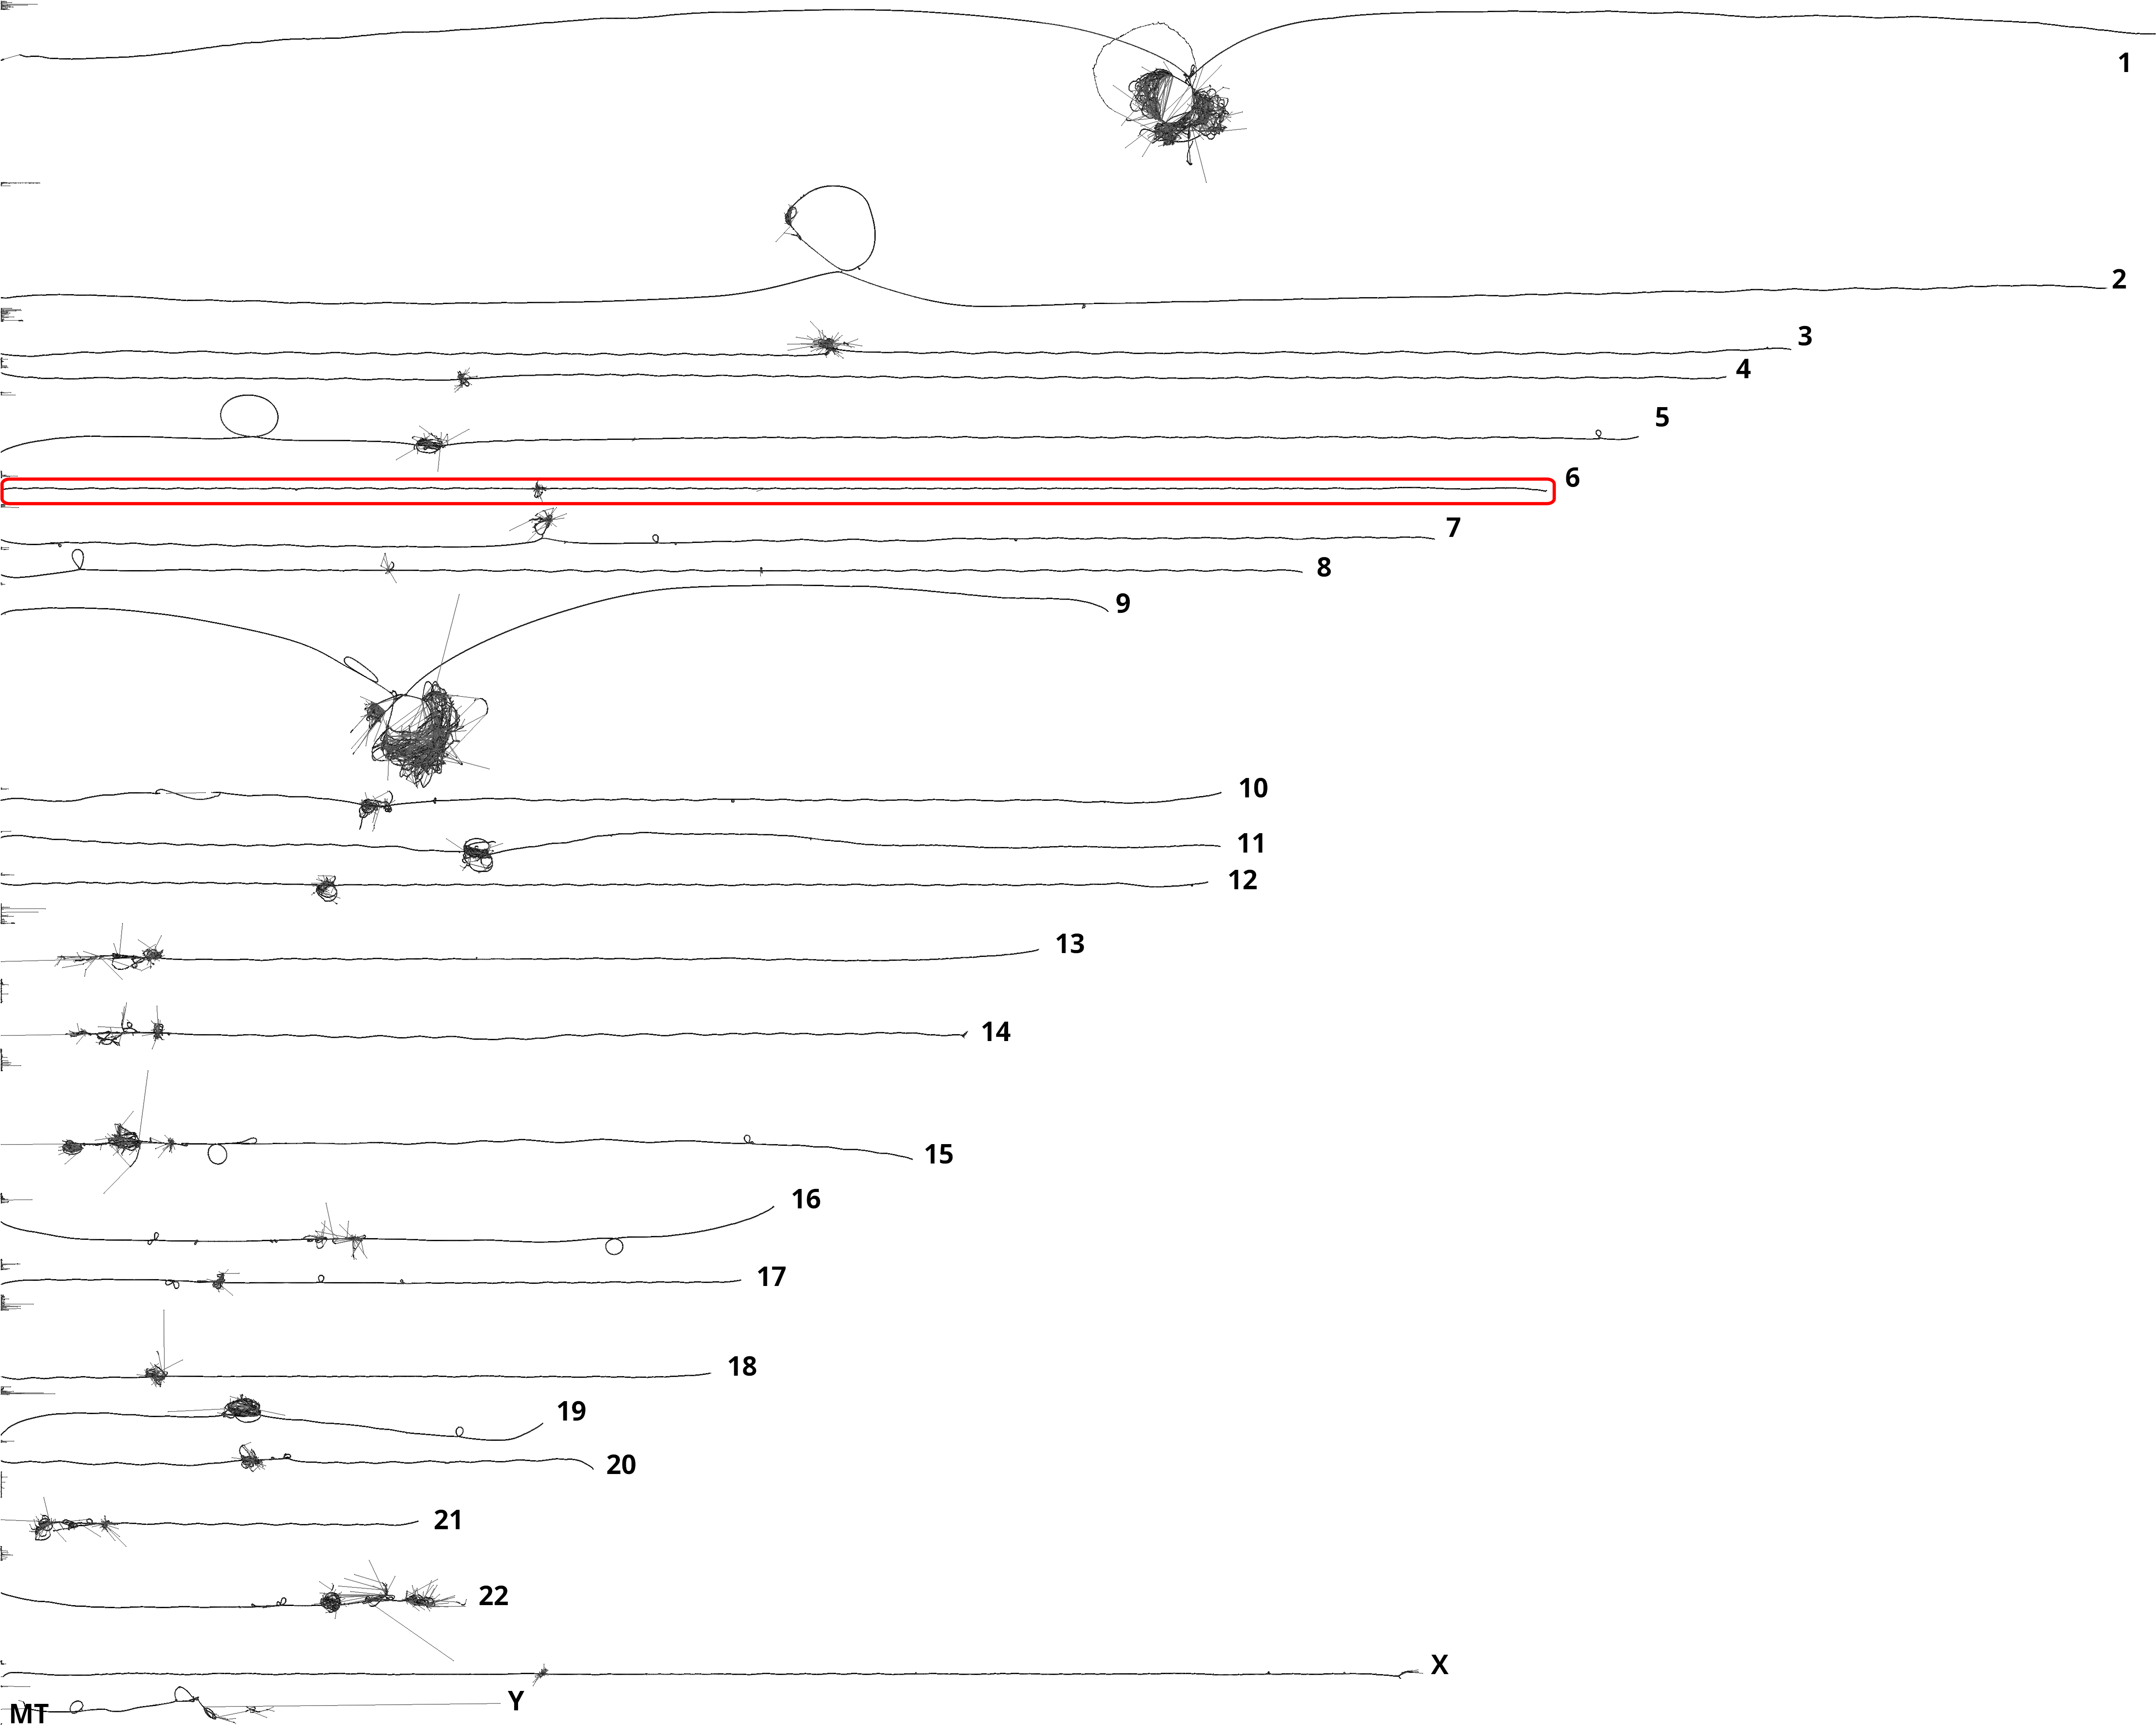
\includegraphics[width=1.0\linewidth]{fig/2D/hprc-v1.0-pggb.og.lay.H4000.r4.0-highlighted.png}
		\label{fig:sfig1}
	\end{subfigure}
	\\
	\begin{subfigure}{1.0\textwidth}
		\centering
		\caption{}
		
\includegraphics[width=1.0\linewidth]{fig/2D/grch38.chr6.MHC_annotated.png}
		\label{fig:sfig2}
	\end{subfigure}
	\\
\begin{subfigure}{1.0\textwidth}
	\centering
	\caption{}
	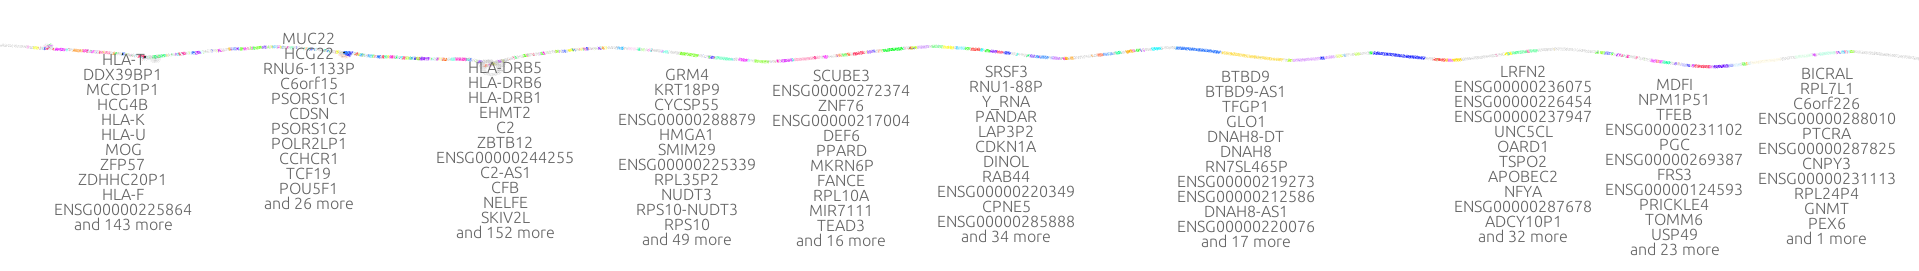
\includegraphics[width=1.0\linewidth]{fig/2D/grch38.chr6.MHC_genes_annotated.png}
	\label{fig:sfig3}
\end{subfigure}
	\\
\begin{subfigure}{1.0\textwidth}
	\centering
	\caption{}
	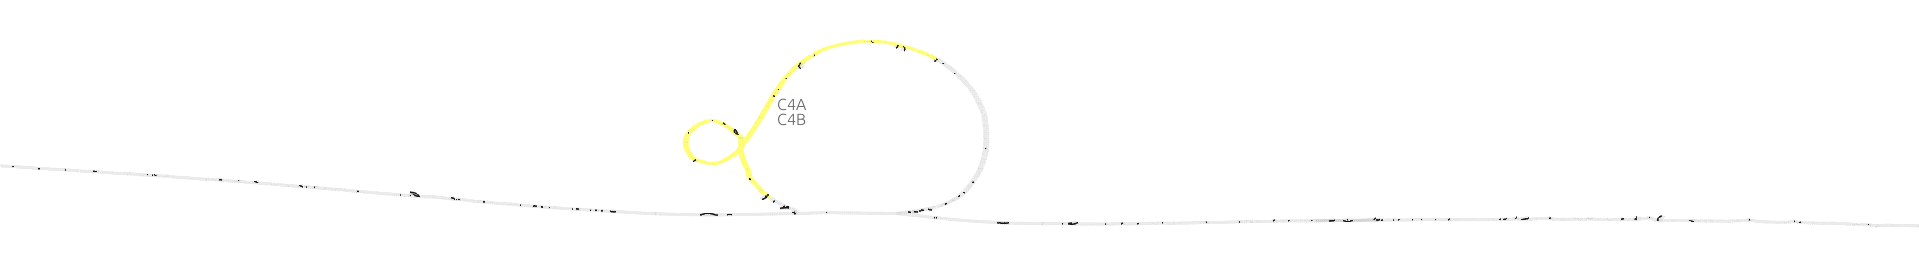
\includegraphics[width=1.0\linewidth]{fig/2D/grch38.chr6.C4_gene_annotated.png}
	\label{fig:sfig4}
\end{subfigure}	
<<<<<<< Updated upstream
	\caption{2D visualizations of all chromosomes of the Human Pangenome Resource Consortium (HPRC) 90 haplotypes pangenome graph, chromosome 6, the major histocompatibility complex (MHC), and the complement component 4 (C4). \textbf{(a)} \textit{odgi draw} layout of the HPRC pangenome graph 90 haplotypes. Displayed are all 24 autosomes and the mitochondrial chromosome. \textbf{(b)} \textit{gfaestus} screenshot of the chromosome 6 layout. Colored in blue is the MHC. \textbf{(c)} \textit{gfaestus} screenshot of the MHC. All MHC genes are color annotated. \textbf{(d)} \textit{gfaestus} screenshot of the region around C4, specifically color highlighting genes C4A and C4B.}
=======
	\caption{2D visualizations of all chromosomes of the Human Pangenome Resource Consortium (HPRC) 90 haplotypes pangenome graph, chromosome 6, the major histocompatibility complex (MHC), and the complement component 4 (C4). 
	\textbf{(a)} \textit{odgi draw} layout of all 24 autosomes and the mitochondrial chromosome. 
	A red rectangle highlights chromosome 6 which is shown in the subfigure below. \textbf{(b)} \textit{gfaestus} screenshot of the chromosome 6 layout. Colored in blue is the MHC. 
	The hairball in the middle is the centromere. 
	The black structures in the centromere are edges. 
	\textbf{(c)} \textit{gfaestus} screenshot of the MHC. 
	All MHC genes are color annotated and the names of the genes appear as a text overlay. \textbf{(d)} \textit{gfaestus} screenshot of the region around C4, specifically color highlighting genes C4A and C4B. 
	The black lines are the edges of the graph.}
>>>>>>> Stashed changes
	\label{fig:2d_layouts}
\end{figure*}
	In Figure~\ref{fig:2d_fig1}, the chromosomes of the HPRC graph show the large scale structural variations in the centromeres.
	Focusing on the major histocompatibility complex (MHC) of chromosome 6 (Figure~\ref{fig:2d_fig2}), the 2D layout reveals the positions and diversity of all MHC genes (Figure~\ref{fig:2d_fig3}).
	In Figure~\ref{fig:2d_fig4} the C4A and C4B genes are highlighted. 
	%The layout is the same as the one produced by \textit{Bandage}~\citep{Wick_2015} and displayed in~\citep{Guarracino2022}.
	Complementary, we provide various 1D visualizations of in Supplementary Figure~\ref{fig:1d_sorts}.

	% \iffalse
	% Fig. 2: Performance evaluation 1D + 2D: Time + RAM by number of haplotypes (Fig.~\ref{fig:haps_time_ram}). Time + RAM by number of threads (Fig.~\ref{fig:threads_time_ram}). Full human graph.
    % \\X
    % 1D (max. threads) vs. ALIBI; we should compare time + RAM in Fig.~\ref{fig:alibi}.
    % But also by our sorting goodness metrics: odgi sort + the one suggested in the ALIBI paper in Table 1.
    % \\
    % 2D (max. threads) + odgi draw vs. Bandage in Fig.~\ref{fig:bandage}.
    % \begin{figure*}[!htb]
	\centering
	%\hline
	\begin{subfigure}[t]{0.4\textwidth}
		\centering
		\caption{}
		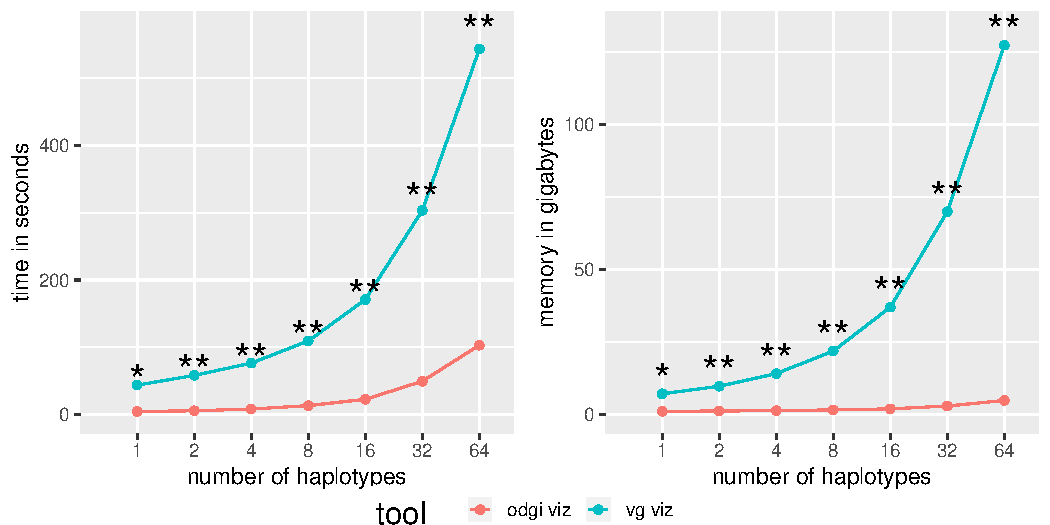
\includegraphics[width=\linewidth]{fig/performance/TODO_by_haps_eval_time_ram.pdf}
		\label{fig:haps_time_ram}
	\end{subfigure}
	\begin{subfigure}[t]{0.4\textwidth}
		\centering
		\caption{}
		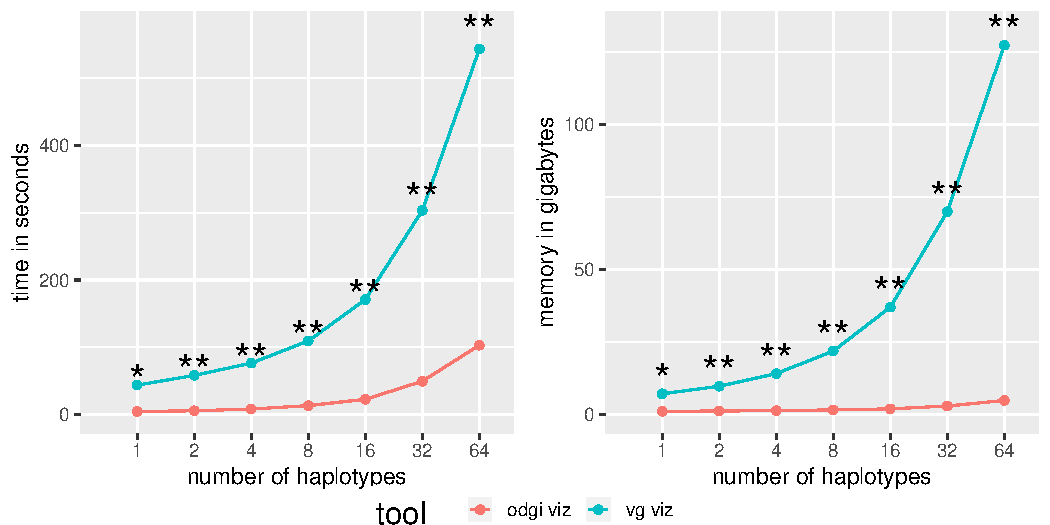
\includegraphics[width=\linewidth]{fig/performance/TODO_by_threads_eval_time_ram.pdf}
		\label{fig:threads_time_ram}
	\end{subfigure}
	%\smallskip
	\begin{subfigure}[t]{0.4\textwidth}
		\centering
		\caption{}
		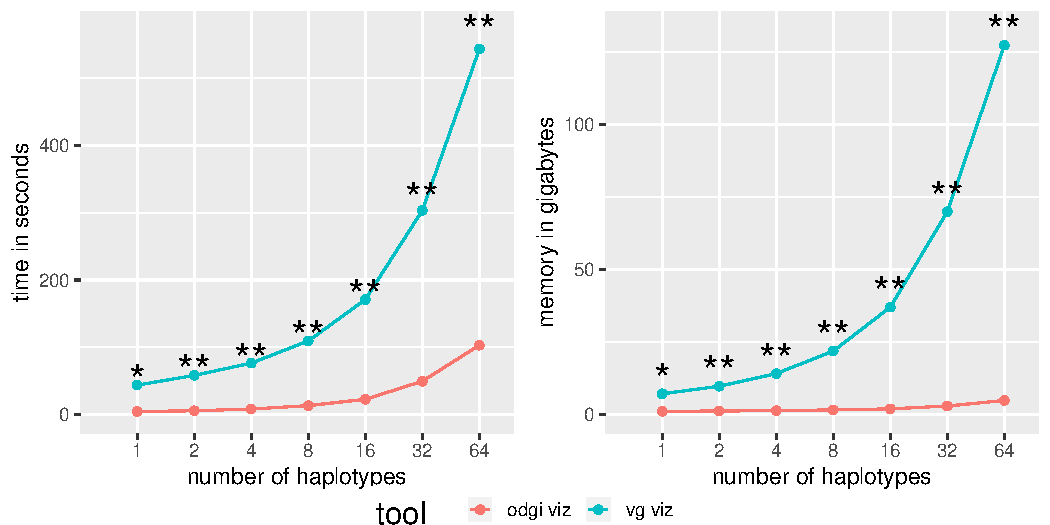
\includegraphics[width=\linewidth]{fig/performance/TODO_1d_alibi_time_ram.pdf}
		\label{fig:alibi}
	\end{subfigure}
	\begin{subfigure}[t]{0.4\textwidth}
		\centering
		\caption{}
		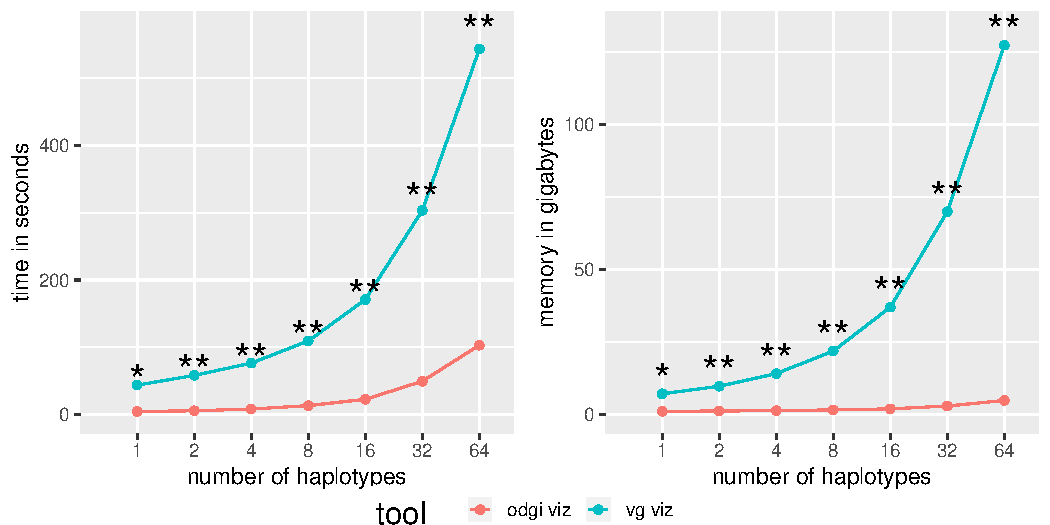
\includegraphics[width=\linewidth]{fig/performance/TODO_by_2d_draw_bandage_time_ram.pdf}
		\label{fig:bandage}
	\end{subfigure}
	\caption{
		Performance evaluations.
		\textbf{(a)} PG-SGD 1D and 2D by haplotypes. \textbf{(b)} PG-SGD 1D and 2D by threads. \textbf{(c)} PG-SGD vs. ALIBI. \textbf{(d)} PG-SGD + draw vs. BANDAGE.
	}
	\label{fig:performance}
\end{figure*}
    % \\
    % \\
    % Table 1: Metrics of the ALIBI and PG-SGD graphs from Fig. 2.
    % \begin{table}[]
	\caption{Metrics of the 1D PG-SGD and ALIBI graphs.}
	\begin{tabular}{|l|l|l|}
		\hline
		& 1D PG-SGD & ALIBI \\ \hline
		METRIC 1 &           &       \\ \hline
		METRIC 2 &           &       \\ \hline
	\end{tabular}
\end{table}
    % Already, PG-SGD outperforms existing graph linearization methods like the flow procedure (\url{https://doi.org/gdw58w}) or ALIBI (\url{https://doi.org/hkv3}).
    % \paragraph{Latent graph structure reveals underlying biology}
    % Fig. 3: Cool quantitative 1D sortings and 2D layouts: biological implications.
    % Randomly sorted. PG-SGD sorted. Ygs sorted. Reference sorted.
    % We want a pipeline of sortings. 2D layout of the whole HPRC.
    % Chr6 HPRC HLA graph? Chr8 beta-defensin gene cluster HPRC? Whole HPRC?
    % \\
    % We could also try to build a gastric cancer pangenome graph with data from \url{https://www.nature.com/articles/s41467-022-33073-7} from up to 185 samples.
    % However, we would have to request access to the data.
    % \\
    % \\
    % \begin{figure*}[!htb]
	\centering
	%\hline
	\begin{subfigure}[t]{0.4\textwidth}
		\centering
		\caption{}
		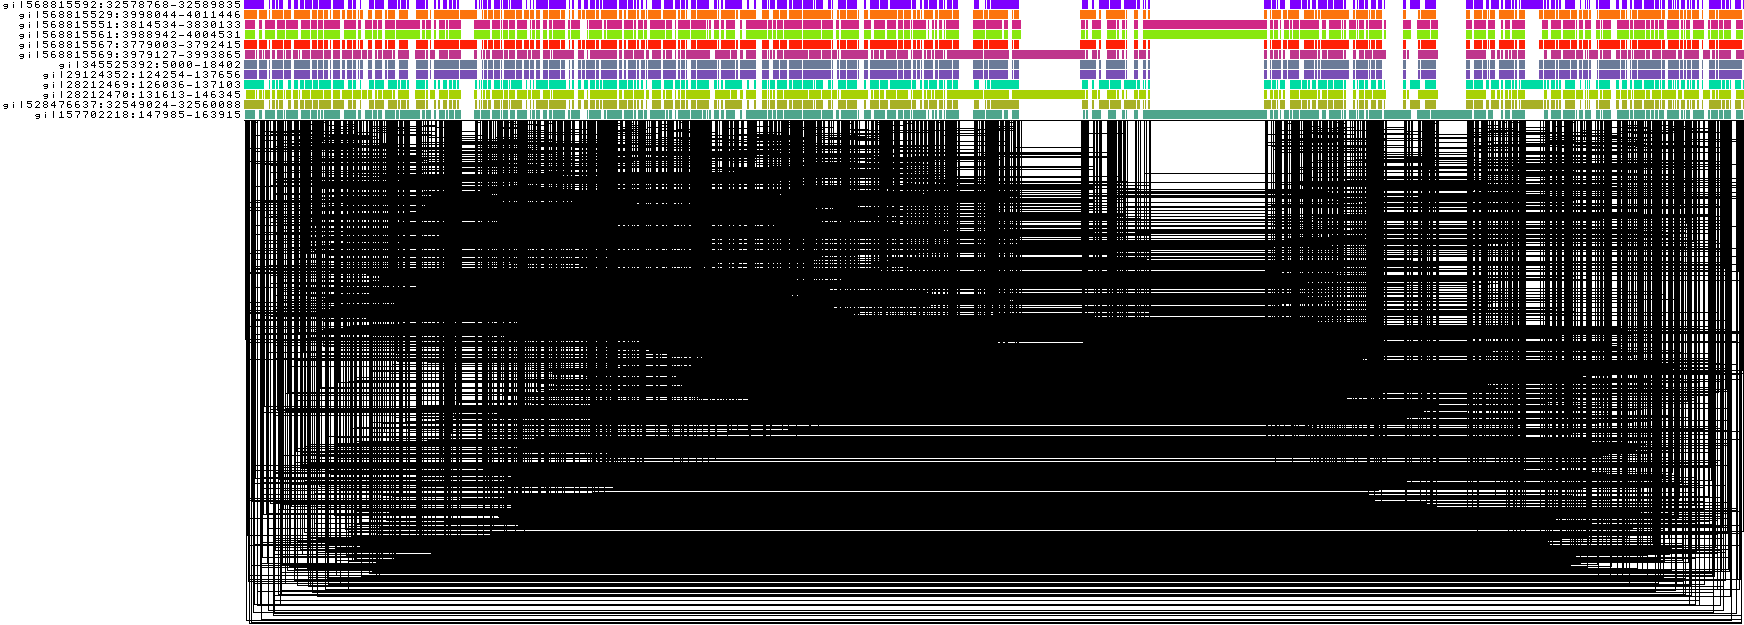
\includegraphics[width=\linewidth]{fig/latent_graph_structure/DRB1-3123.fa.gz.c666522.417fcdf.seqwish.og.r.og.png}
		\label{fig:random}
	\end{subfigure}
	\begin{subfigure}[t]{0.4\textwidth}
		\centering
		\caption{}
		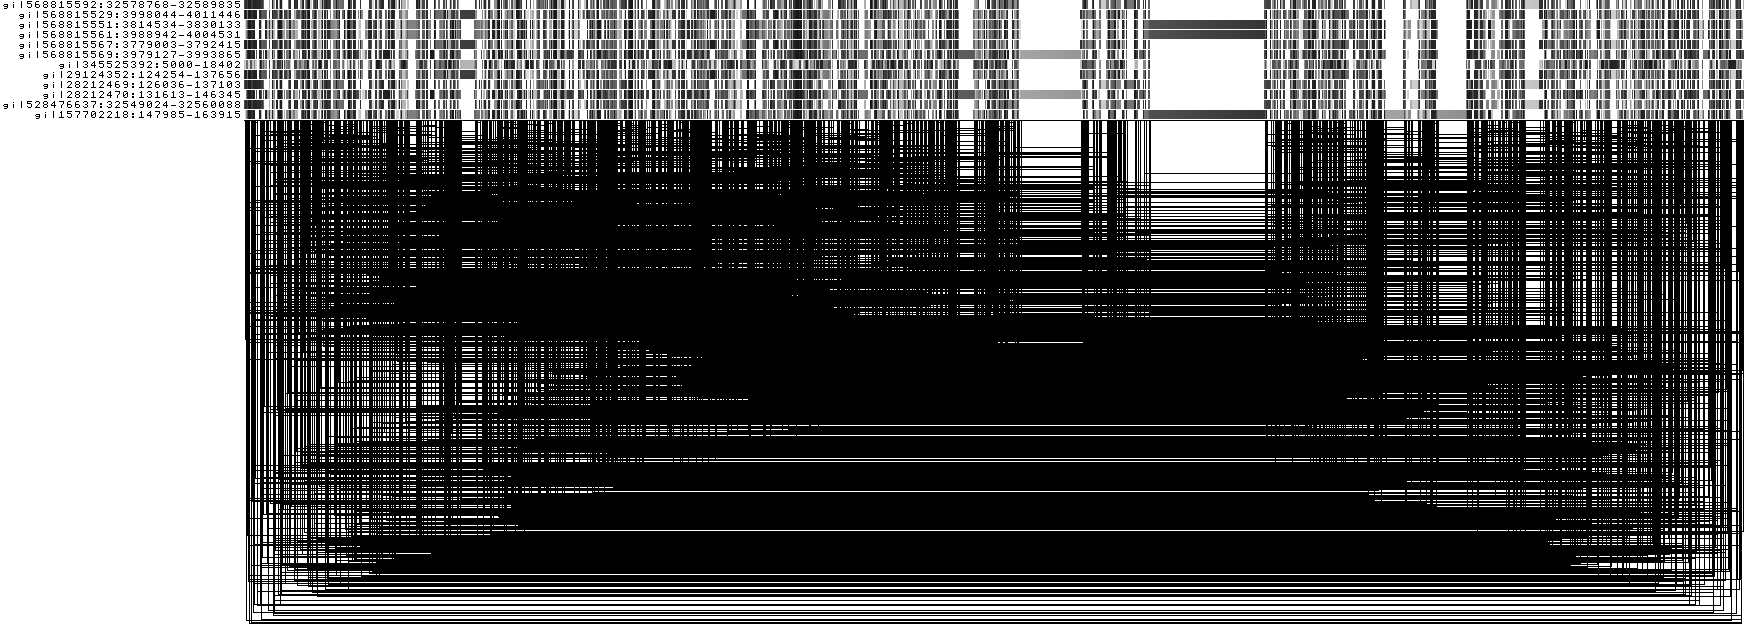
\includegraphics[width=\linewidth]{fig/latent_graph_structure/DRB1-3123.fa.gz.c666522.417fcdf.seqwish.og.r.og.ud.png}
		\label{fig:random_pos}
	\end{subfigure}
	%\smallskip
	\begin{subfigure}[t]{0.4\textwidth}
		\centering
		\caption{}
		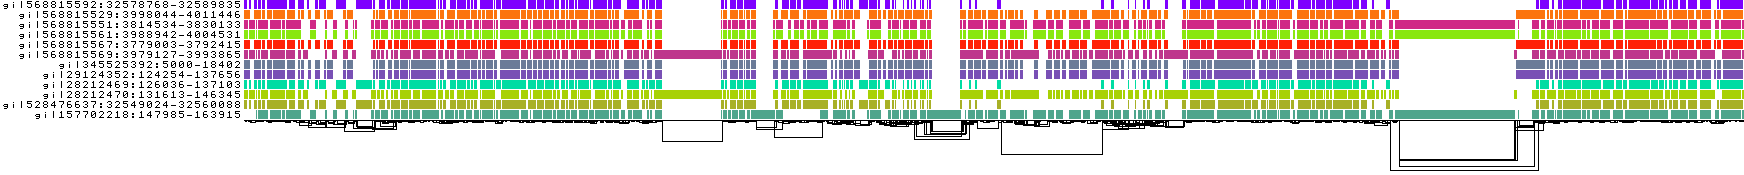
\includegraphics[width=\linewidth]{fig/latent_graph_structure/DRB1-3123.fa.gz.c666522.417fcdf.seqwish.og.Y.og.png}
		\label{fig:sorted}
	\end{subfigure}
	\begin{subfigure}[t]{0.4\textwidth}
		\centering
		\caption{}
		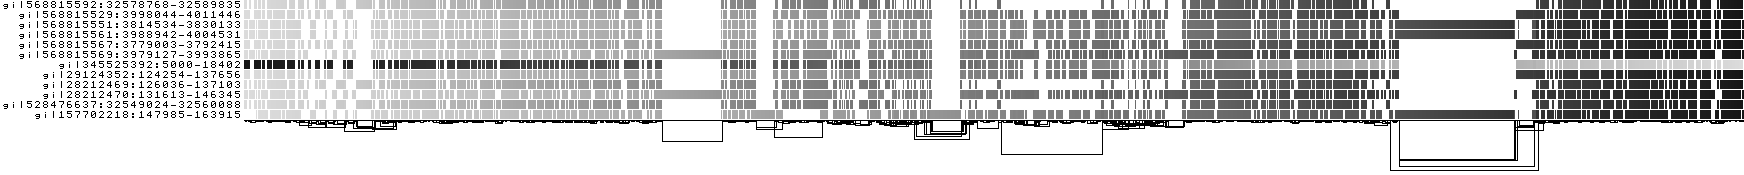
\includegraphics[width=\linewidth]{fig/latent_graph_structure/DRB1-3123.fa.gz.c666522.417fcdf.seqwish.og.Y.og.ud.png}
		\label{fig:sorted_pos}
	\end{subfigure}
	\begin{subfigure}[t]{0.4\textwidth}
		\centering
		\caption{}
		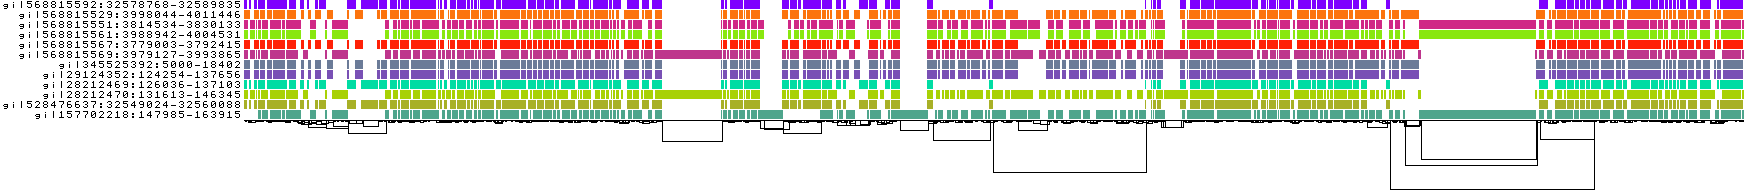
\includegraphics[width=\linewidth]{fig/latent_graph_structure/DRB1-3123.fa.gz.c666522.417fcdf.seqwish.og.Ygs.og.png}
		\label{fig:pipeline}
	\end{subfigure}
	\begin{subfigure}[t]{0.4\textwidth}
		\centering
		\caption{}
		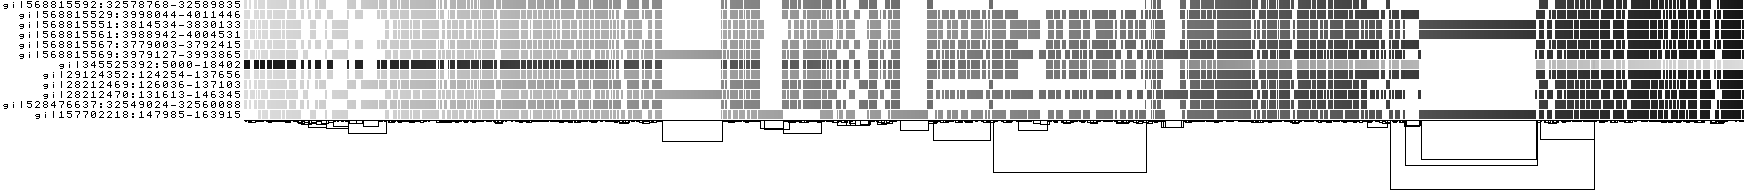
\includegraphics[width=\linewidth]{fig/latent_graph_structure/DRB1-3123.fa.gz.c666522.417fcdf.seqwish.og.Ygs.og.ud.png}
		\label{fig:pipeline_pos}
	\end{subfigure}
	\begin{subfigure}[t]{0.4\textwidth}
		\centering
		\caption{}
		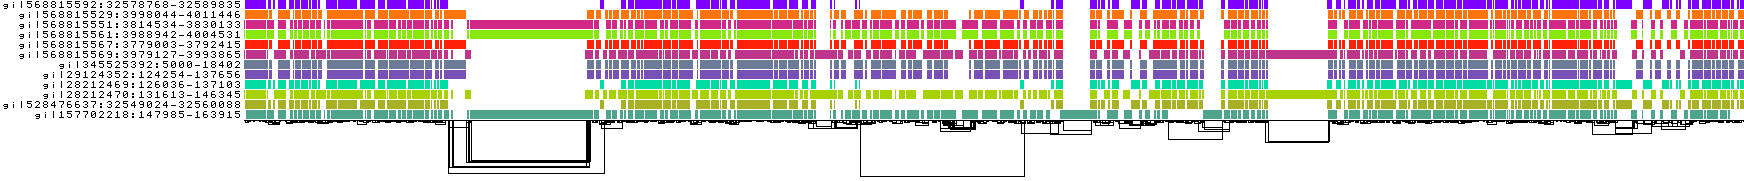
\includegraphics[width=\linewidth]{fig/latent_graph_structure/DRB1-3123.fa.gz.c666522.417fcdf.seqwish.og.YH.og.png}
		\label{fig:ref}
	\end{subfigure}
	\begin{subfigure}[t]{0.4\textwidth}
		\centering
		\caption{}
		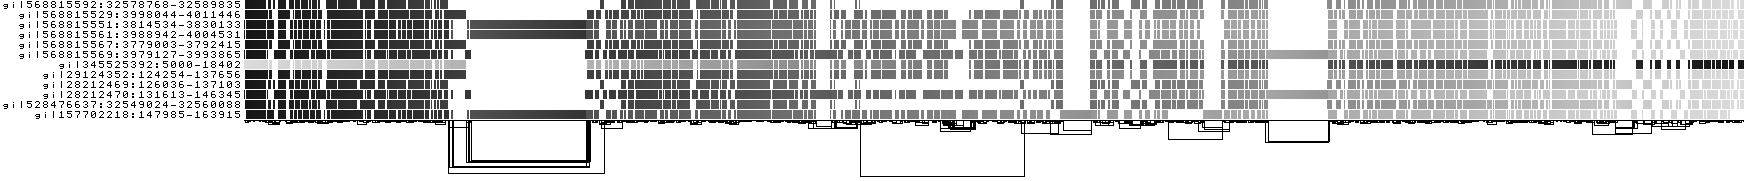
\includegraphics[width=\linewidth]{fig/latent_graph_structure/DRB1-3123.fa.gz.c666522.417fcdf.seqwish.og.YH.og.ud.png}
		\label{fig:ref_pos}
	\end{subfigure}
		\begin{subfigure}[t]{0.8\textwidth}
		\centering
		\caption{}
		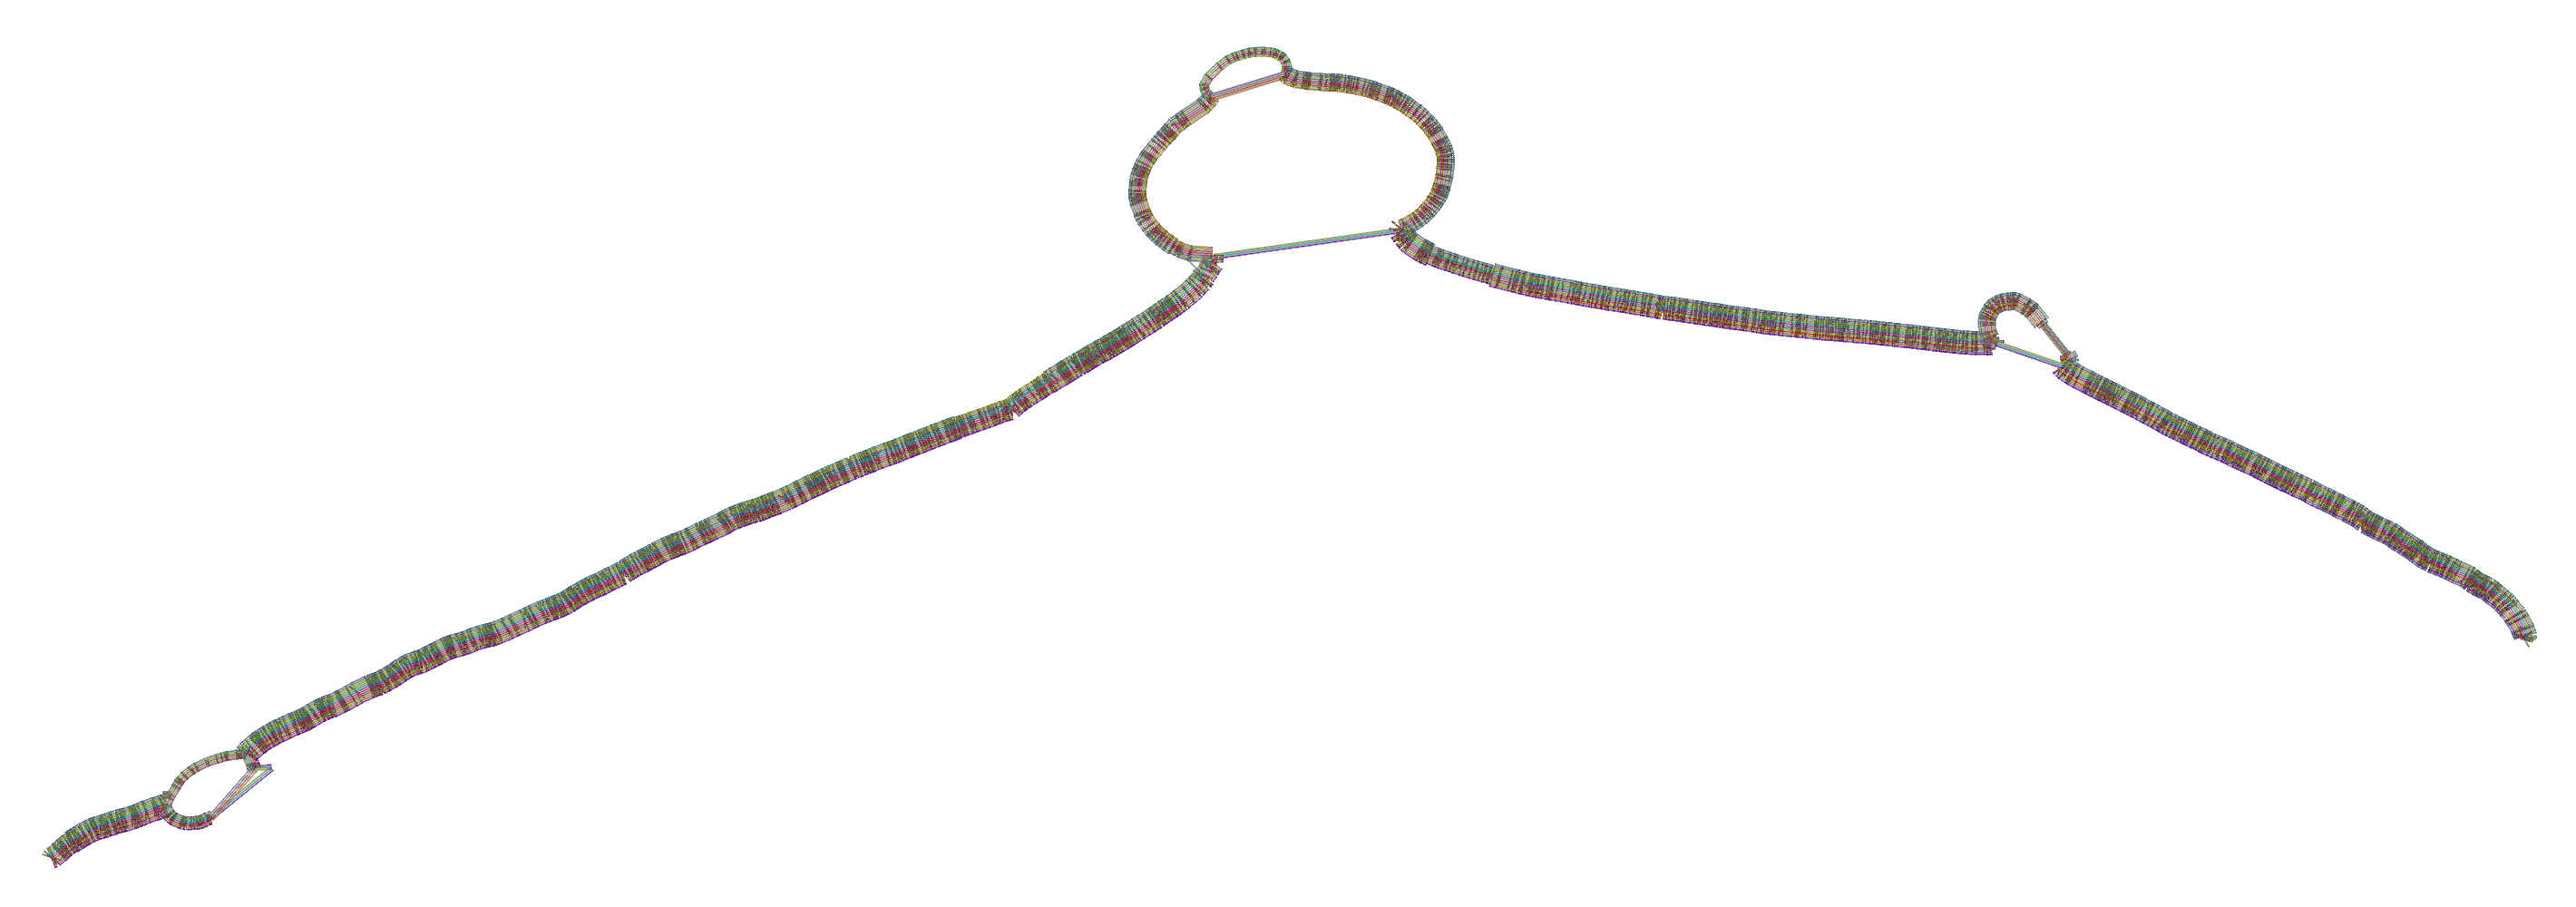
\includegraphics[width=\linewidth]{fig/latent_graph_structure/TODO_2d.png}
		\label{fig:2d}
	\end{subfigure}
	\caption{
		Latent graph structures.
		\textbf{(a)} Randomly sorted graph. \textbf{(b)} Randomly sorted graph by position. \textbf{(c)} PG-SGD sorted graph. \textbf{(d)} PG-SGD sorted graph by position. \textbf{(e)} Ygs sorted graph. \textbf{(f)} Ygs sorted graph by position. \textbf{(g)} Reference sorted graph. \textbf{(h)} Reference sorted graph by position. \textbf{(i)} 2D layout of graph.
	}
	\label{fig:latent_graph_structure}
\end{figure*}
    % Table 2: Metrics of the sorted graphs in Fig. 3.
    % \begin{table}[]
	\caption{Metrics of the latent graphs.}
	\begin{tabular}{|l|l|l|l|l|}
		\hline
		& RANDOM & Y & Ygs & Ref \\ \hline
		METRIC 1 &        &   &     &     \\ \hline
		METRIC 2 &        &   &     &     \\ \hline
	\end{tabular}
\end{table}
    % \paragraph{Bonus Section}
    % Fig. 4: Detect tension. Relax a graph. Detect tension afterwards.
    % I need to test this on a new data set I got from Erik.
    % I need to establish a fixed lower boundary for the tension from which on we don't relax anymore. \\
    % With a high quality layout, we can measure the discrepancy of the path layout position versus the expected path nucleotide position, the “tension” of a graph.
    % The greater the “tension”, the greater is the possibility of a biologically meaningless alignment.
    % This allows us to detect telomere collapsing alignment errors and hopefully (pangenome) assembly errors, subsequently correcting them.
    % \begin{figure*}[!htb]
	\centering
	%\hline
	\begin{subfigure}[t]{0.4\textwidth}
		\centering
		\caption{}
		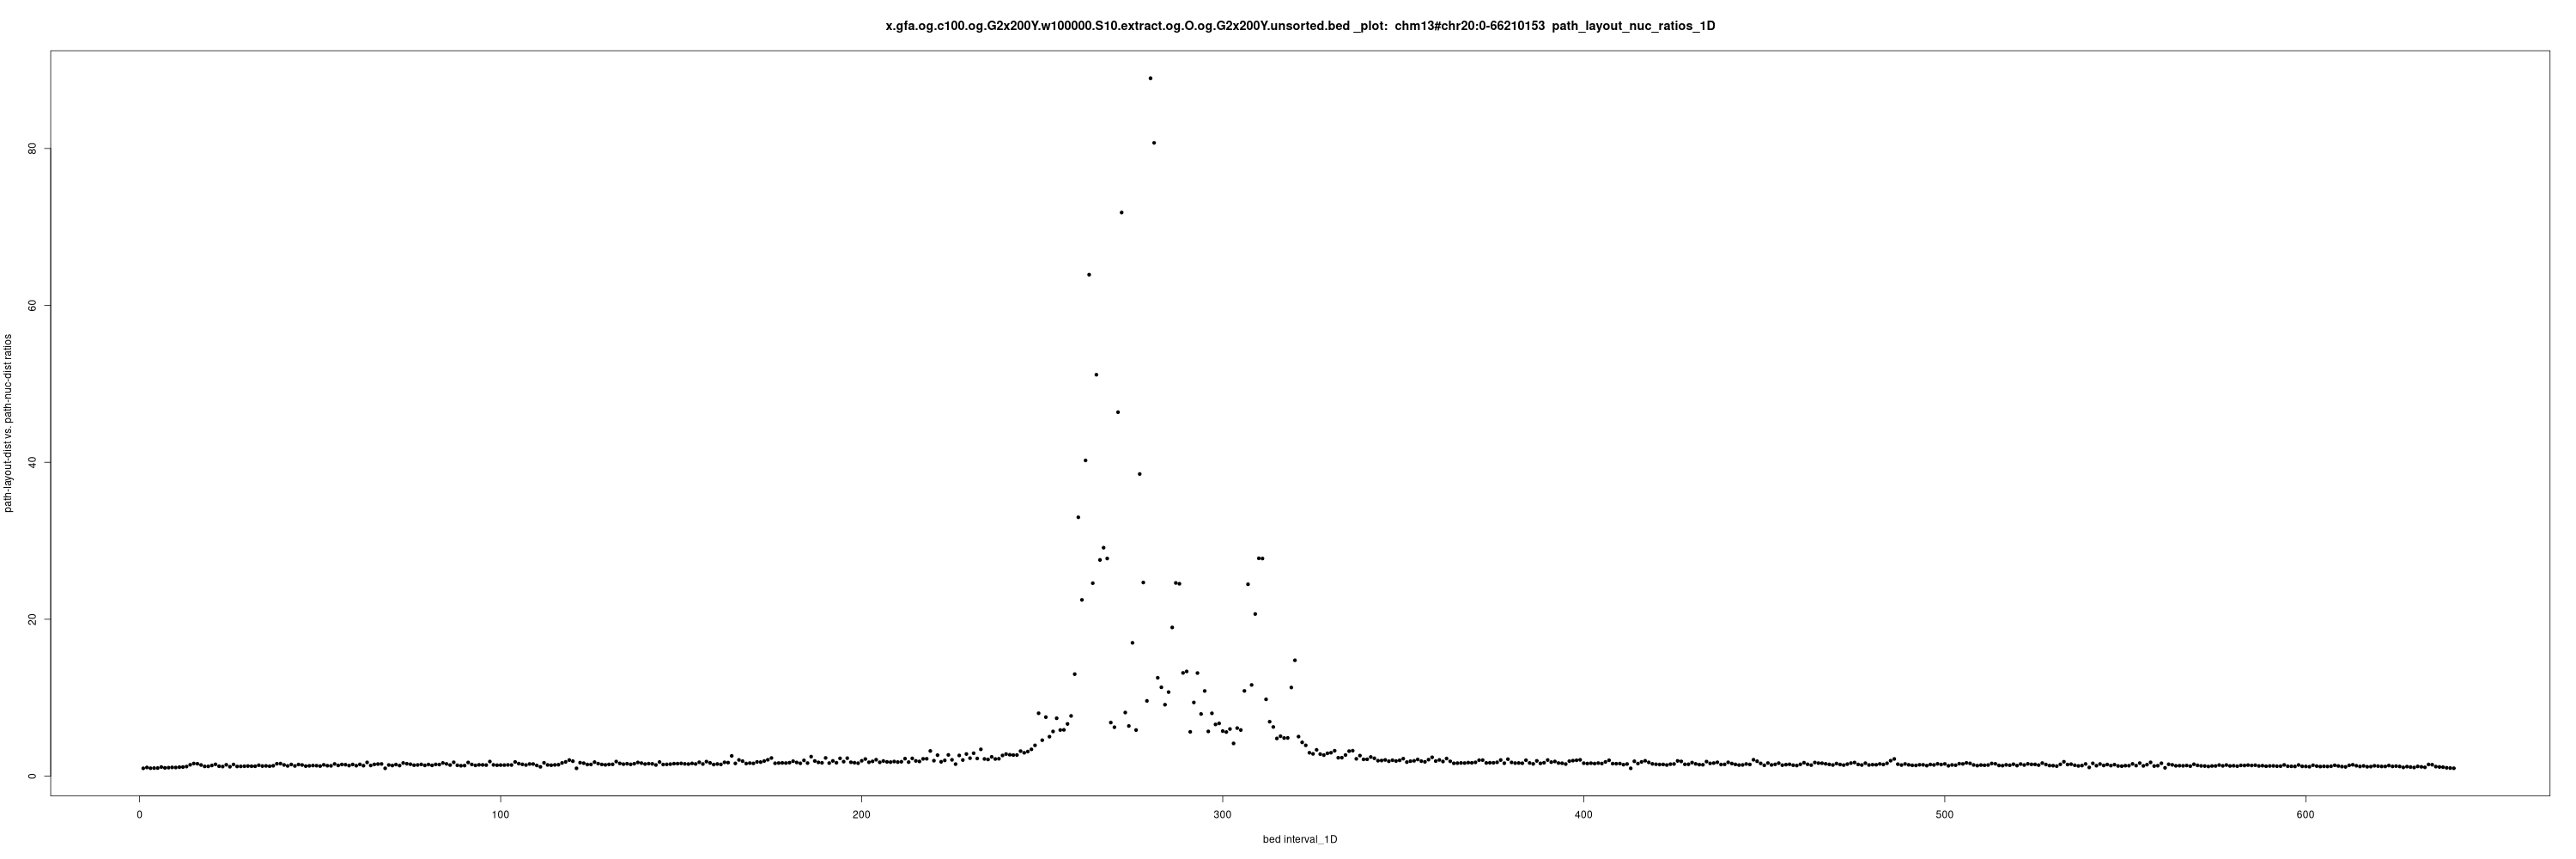
\includegraphics[width=\linewidth]{fig/tension/tension_bed.png}
		\label{fig:tension_bed}
	\end{subfigure}
	\begin{subfigure}[t]{0.4\textwidth}
		\centering
		\caption{}
		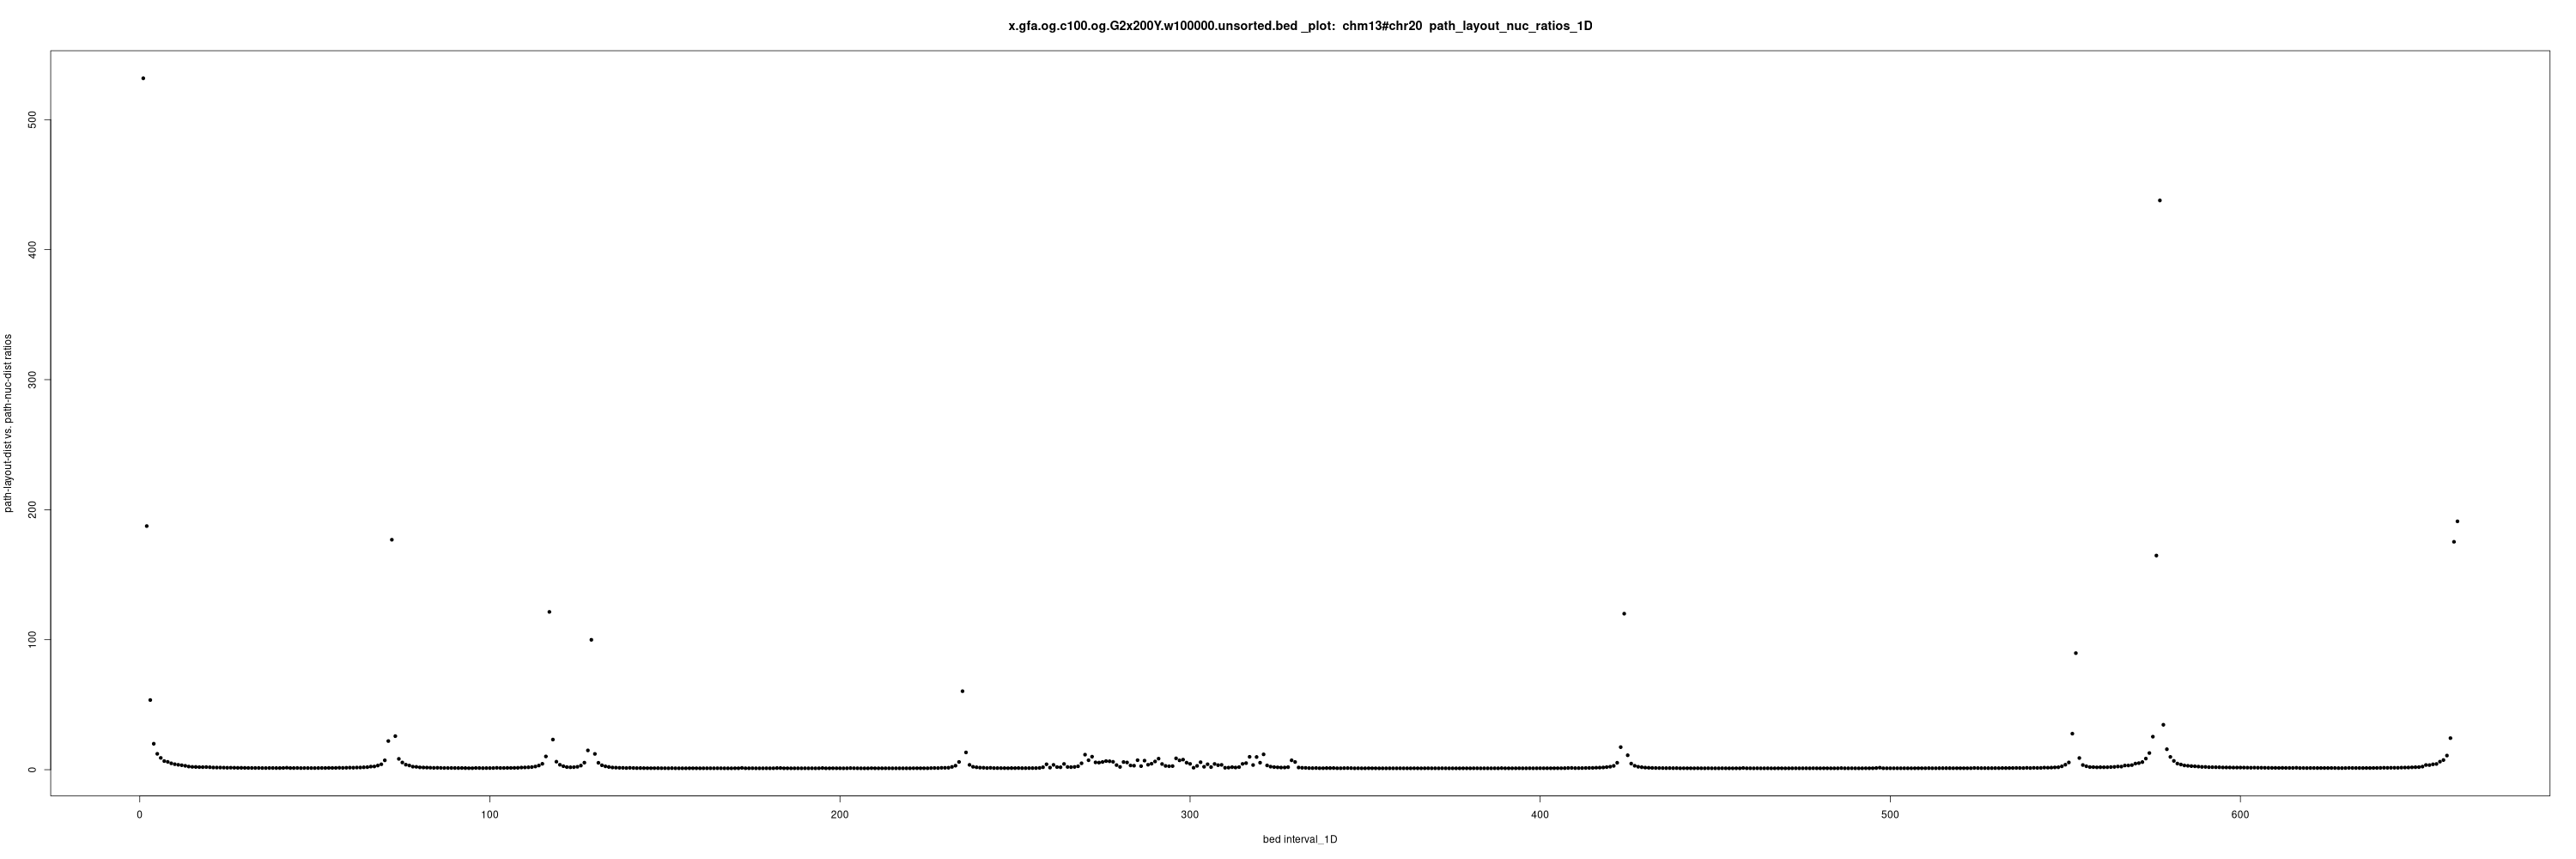
\includegraphics[width=\linewidth]{fig/tension/tension_bed_relaxed.png}
		\label{fig:tension_extracted}
	\end{subfigure}
\\
	%\smallskip
	\begin{subfigure}[t]{0.1\textwidth}
		\centering
		\caption{}
		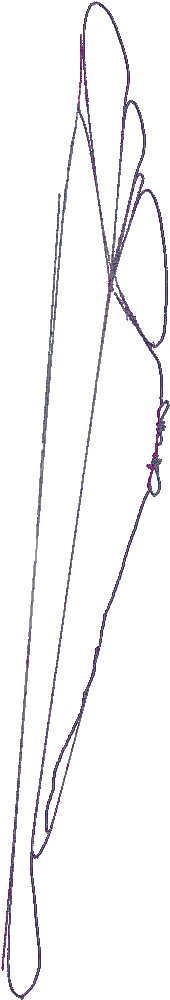
\includegraphics[width=\linewidth]{fig/tension/layout.png}
		\label{fig:tension_draw}
	\end{subfigure}
	\begin{subfigure}[t]{0.1\textwidth}
		\centering
		\caption{}
		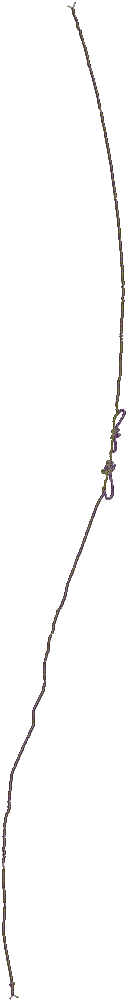
\includegraphics[width=\linewidth]{fig/tension/layout_relaxed.png}
		\label{fig:tension_draw_extracted}
	\end{subfigure}
	\caption{
		Detecting tension and relaxing a pangenome graph.
		\textbf{(a)} Tension detection before relaxation. \textbf{(b)} Tension detection after relaxation. \textbf{(c)} Folded 2D before relaxation. \textbf{(d)} Linearized 2D after relaxation.
	}
	\label{fig:tension}
\end{figure*}
    % \fi

	\section{Discussion}
	\label{sec:discussion}
	
	We presented Path-Guided Stochastic Gradient Descent (PG-SGD), the first layout algorithm for pangenome graphs that leverages the biological information available within the genomes represented in the graph.
	Our implementation efficiently computes the layout of pangenome graphs representing thousands of whole genomes.
	
	Graph visualization is key for understanding genome variations and the layouts produced by PG-SGD offer an unprecedented high-level perspective on pangenome variation.
	We implemented PG-SGD to generate layouts in 1D and 2D.
	These graph projections have already been employed in constructing and analyzing the first draft human pangenome reference \citep{Liao2023}, as well as in the discovery of heterologous recombination of human acrocentric chromosomes \citep{Guarracino2023}.
	Furthermore, they are applied in the creation and analysis of pangenome graphs for any species \citep{Guarracino2022, Garrison2023}.
	%The graph simplification pipeline smoothxg runs POA for each block of paths that are co-linear within each seqwish induced variation graph.
	%A prerequisite is that the graph nodes are sorted according to their occurrence in the graph's embedded paths.
	%Our 1D path-guided SGD algorithm is designed to provide this kind of sort.
	Of note, there still remains a gap in interactive and scalable solutions that merge layouts of large pangenome graph with annotation.
	Our algorithm will underpin new pangenome graph browsers for studying graph layouts and the genome variation they represent (\url{https://github.com/chfi/waragraph)} last accessed Jul 2023).
	
	% \FIXME{@Jiajie + Niklas: Maybe address our SMT issue with your cache locality as a potential solution. Additionally just 2/3 sentences about going GPU?}
	The performance analysis shows that our 2D implementation outperforms \textit{BandageNG} when handling large, complex pangenome graphs.
	While \textit{BandageNG} was not able to deliver a layout of the whole HPRC graph within 1 week, our 2D PG-SGD calculated one within one day.
	%We expect that our implementation will be able to handle the next phase of the HPRC, 24 chromosomal pangenome graphs constructed from 300 individuals, without any problems.
	There are some possible optimization approaches for future work to further improve the performance of PG-SGD, making it possible for interactive use. 
	The data structure could be optimized to improve ache performance. Moreover, the high-degree of parallelism could be further exploited by using a GPU.  
	% As especially observed with chromosome 16 evaluation, our implementation is memory-bound.
	% The current data structure doesn't consider the memory access pattern.
	% Therefore, a CPU cache optimized implementation could make use of the massive parallelized calculations on a GPU.
	% Such efforts are currently in progress \url{https://github.com/nsmlzl/odgi/tree/layout_cache_optimized_cpu}.

	PG-SGD can be extended to any number of dimensions.
	It can be seen as a graph embedding algorithm that converts high-dimensional, sparse pangenome graphs into low-dimensional, dense, and continuous vector spaces, while preserving its biologically relevant information.
	This enables the application of machine learning algorithms that use the graph layout for variant detection and classification. 
	Our future research involves leveraging these graph projections to detect structural variants and to identify and correct assembly errors. 
	Moreover, we are considering extending the algorithm to RNA and protein sequences to support pantranscriptome graphs \citep{sibbesen_haplotype-aware_2023} and panproteome graphs \citep{dabbaghie_panpa:_2023}, respectively.
	%Helpful could be to integrate more layout objectives \citep{ahmed_multicriteria_2021} like neighborhood preservation.

	\section*{Acknowledgments}

	We thank Matthias Seybold from the Quantitative Biology Center for maintaining the Core Facility Cluster.
	
	\section*{Funding}
	
	S.H. acknowledges funding from the Central Innovation Programme (ZIM) for SMEs of the Federal Ministry for Economic Affairs and Energy of Germany.
	S.N. acknowledges Germany’s Excellence Strategy (CMFI), EXC-2124 and (iFIT)—EXC 2180–390900677.
	This work was supported by the BMBF-funded de.NBI Cloud within the German Network for Bioinformatics Infrastructure (de.NBI) (031A532B, 031A533A, 031A533B, 031A534A, 031A535A, 031A537A, 031A537B, 031A537C, 031A537D and 031A538A).
	A.G. acknowledges efforts by Nicole Soranzo to establish a pangenome research unit at the Human Technopole in Milan, Italy.
	JNM.S., J.L., Z.Z., P.P., and E.G. acknowledge funding from the NSF PPoSS Award \#2118709.
	
	\section*{Competing interests}
	Author J.H. is employed by Computomics GmbH.
	
	\section*{Software and data availability}
	
	Software versions, code, and links to data resources used to prepare this manuscript can be found at \url{https://github.com/pangenome/sorting-paper}.
	Animations of the algorithm are deposited at \url{https://doi.org/10.5281/zenodo.8288999}.
		
	\bibliographystyle{natbib}
	
	\bibliography{document}
	
	\clearpage
	\setcounter{page}{1}
	
	\beginsupplement
	
	\section{Supplement}
	
	 \subsection{Supplementary data}
	 %\subsection{Quantization} % DURING REVISION, IF NEEDED
	 %More details about your clever quantization.
	 \subsubsection{Performance evaluation}
	 \label{sec:performance}
	 The results of the performance evaluation are given in Table~\ref{tab:layout}.
	 \begin{table*}[!ht]
	\centering
	\ra{1.2}
	\caption{\label{tab:layout} Performance evaluation of computing a 2D layout of all chromosomal HPRC pangenome graphs. From GFA to the actual layout.}
	\begin{tabular}{@{}lrrrrrrrrr@{}}
		& & & & & &  \multicolumn{2}{c}{$\mathbf{time\ in\ minutes}$}  & \multicolumn{2}{c}{$\mathbf{memory\ in\ gigabytes}$}\\ \cmidrule(lr){7-8} \cmidrule(lr){9-10}
		{$\mathbf{name}$} & {$\mathbf{len}$} & {$\mathbf{nodes}$} & {$\mathbf{edges}$} & {$\mathbf{paths}$} & {$\mathbf{steps}$} & {$\mathbf{pg-sgd}$} & {$\mathbf{bng}$} & {$\mathbf{pg-sgd}$} & {$\mathbf{bng}$}\\ \hline
		chr1 & 1.12e+09 & 1.11e+07 & 1.54e+07 & 2.26e+03 & 6.01e+08 & \textbf{68} & 1427 & \textbf{56.00} & 195.33 \\ 
		chr2 & 3.47e+08 & 6.68e+06 & 9.27e+06 & 1.65e+03 & 3.89e+08 & \textbf{47} & 521 & \textbf{37.29} & 81.97 \\ 
		chr3 & 4.06e+08 & 6.20e+06 & 8.62e+06 & 1.56e+03 & 4.55e+08 & \textbf{52} & 481 & \textbf{41.71} & 93.83 \\ 
		chr4 & 2.73e+08 & 5.91e+06 & 8.23e+06 & 1.35e+03 & 4.97e+08 & \textbf{56} & 423 & \textbf{45.02} & 79.48 \\ 
		chr5 & 3.35e+08 & 5.39e+06 & 7.51e+06 & 1.20e+03 & 4.04e+08 & \textbf{46} & 375 & \textbf{36.48} & 75.10 \\ 
		chr6 & 2.29e+08 & 4.70e+06 & 6.56e+06 & 1.41e+03 & 4.03e+08 & \textbf{46} & 271 & \textbf{37.22} & 71.26 \\ 
		chr7 & 2.71e+08 & 5.17e+06 & 7.25e+06 & 1.22e+03 & 4.10e+08 & \textbf{46} & 346 & \textbf{37.88} & 73.81 \\ 
		chr8 & 1.93e+08 & 4.26e+06 & 5.95e+06 & 8.55e+02 & 4.29e+08 & \textbf{47} & 233 & \textbf{38.07} & 54.70 \\ 
		chr9 & 1.01e+09 & 8.80e+06 & 1.23e+07 & 8.67e+02 & 3.31e+08 & \textbf{38} & 957 & \textbf{31.79} & 131.96 \\ 
		chr10 & 2.56e+08 & 4.50e+06 & 6.26e+06 & 8.79e+02 & 2.72e+08 & \textbf{32} & 260 & \textbf{25.25} & 67.87 \\ 
		chr11 & 2.83e+08 & 4.73e+06 & 6.54e+06 & 6.53e+02 & 2.38e+08 & \textbf{28} & 286 & \textbf{21.77} & 68.54 \\ 
		chr12 & 2.44e+08 & 4.10e+06 & 5.71e+06 & 7.68e+02 & 2.54e+08 & \textbf{27} & 206 & \textbf{23.99} & 51.22 \\ 
		chr13 & 3.47e+08 & 4.34e+06 & 6.08e+06 & 2.58e+03 & 3.12e+08 & \textbf{34} & 237 & \textbf{28.64} & 85.85 \\ 
		chr14 & 2.73e+08 & 4.15e+06 & 5.79e+06 & 1.82e+03 & 2.62e+08 & \textbf{28} & 222 & \textbf{24.17} & 78.13 \\ 
		chr15 & 5.64e+08 & 5.20e+06 & 7.26e+06 & 2.06e+03 & 4.02e+08 & \textbf{35} & 334 & \textbf{35.69} & 102.97 \\ 
		chr16 & 3.39e+08 & 3.91e+06 & 5.53e+06 & 1.52e+03 & 6.91e+08 & 512 & \textbf{244} & 61.02 & \textbf{53.00} \\ 
		chr17 & 1.73e+08 & 2.76e+06 & 3.93e+06 & 1.42e+03 & 3.25e+08 & \textbf{33} & 102 & \textbf{28.69} & 49.50 \\ 
		chr18 & 2.44e+08 & 2.83e+06 & 3.98e+06 & 1.27e+03 & 3.00e+08 & \textbf{31} & 106 & \textbf{26.78} & 45.01 \\ 
		chr19 & 2.91e+08 & 3.02e+06 & 4.21e+06 & 1.07e+03 & 2.03e+08 & \textbf{21} & 117 & \textbf{18.43} & 40.18 \\ 
		chr20 & 1.87e+08 & 2.82e+06 & 3.97e+06 & 8.24e+02 & 2.35e+08 & \textbf{25} & 108 & \textbf{21.04} & 39.05 \\ 
		chr21 & 2.74e+08 & 2.76e+06 & 3.88e+06 & 3.03e+03 & 2.21e+08 & \textbf{23} & 103 & \textbf{19.12} & 46.47 \\ 
		chr22 & 4.64e+08 & 3.76e+06 & 5.22e+06 & 1.76e+03 & 2.05e+08 & \textbf{22} & 183 & \textbf{18.65} & 45.13 \\ 
		chrX & 2.07e+08 & 3.46e+06 & 4.89e+06 & 2.42e+03 & 2.70e+08 & \textbf{28} & 155 & \textbf{24.84} & 43.05 \\ 
		chrY & 8.80e+07 & 3.18e+05 & 4.41e+05 & 3.07e+02 & 1.34e+07 & \textbf{1} & 5 & \textbf{1.57} & 4.65 \\ 
		chrM & 1.76e+04 & 1.40e+03 & 1.89e+03 & 4.40e+01 & 4.06e+04 & \textbf{1} & \textbf{1} & 0.49 & \textbf{0.04}  \\ 
		all chrs & 8.42e+09 & 1.11e+08 & 1.55e+08 & 3.48e+04 & 8.12e+09 & \textbf{1020} & ?  & \textbf{738.76} & ? ($\approx$1567.45)\\
		\bottomrule
	\end{tabular}
\end{table*}
	 %\FIXME{What about the SMT thingy?} % DURING REVISION, IF NEEDED
	\subsubsection{1D visualizations}	
	The 1D PG-SGD algorithm creates a 1D layout of the nodes of the graph.
	Theoretically, it is possible that 2 nodes have the same 1D coordinate or overlap.
	But, in our 1D visualizations, we arrange the nodes from left to right.
	Therefore, we project the 1D coordinates into a 1D node order: We sort the final layout by graph component, graph position, and node rank.
	\begin{figure*}[!htpb]
	\centering
	\begin{subfigure}{1.0\textwidth}
		\centering
		\caption{}
		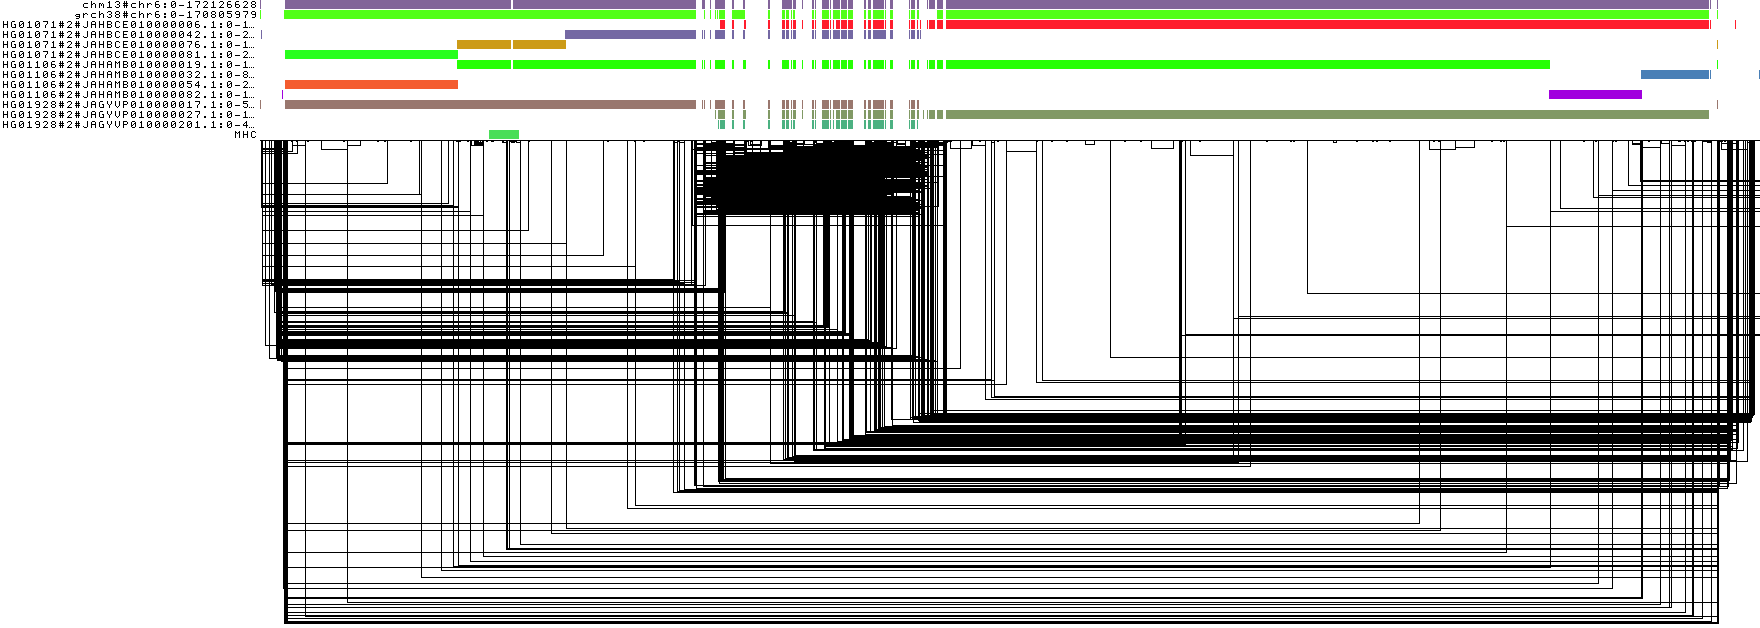
\includegraphics[width=1.0\linewidth]{fig/1D/chr6.hprc-v1.0-pggb.13paths.MHC.og.png}
		\label{fig:1d_fig1}
	\end{subfigure}
	\\
	\begin{subfigure}{1.0\textwidth}
		\centering
		\caption{}
		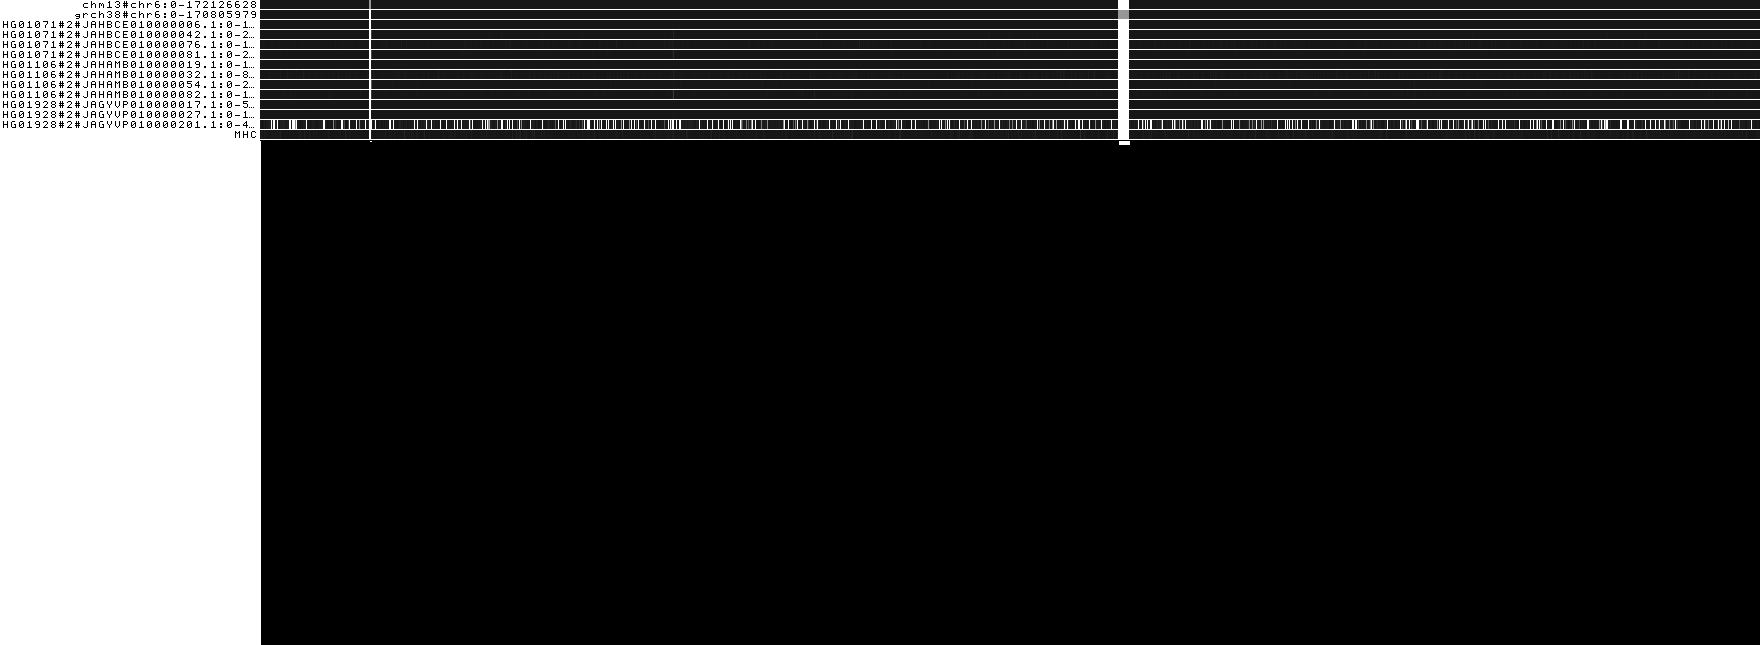
\includegraphics[width=1.0\linewidth]{fig/1D/chr6.hprc-v1.0-pggb.13paths.MHC.og.r.og.png}
		\label{fig:1d_fig2}
	\end{subfigure}
	\\
	\begin{subfigure}{1.0\textwidth}
		\centering
		\caption{}
		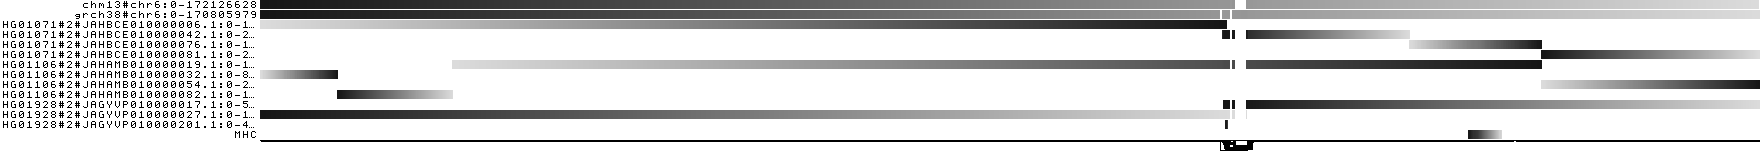
\includegraphics[width=1.0\linewidth]{fig/1D/chr6.hprc-v1.0-pggb.13paths.MHC.og.r.og.Y.og.png}
		\label{fig:1d_fig3}
	\end{subfigure}
	\\
	\begin{subfigure}{1.0\textwidth}
		\centering
		\caption{}
		
\includegraphics[width=1.0\linewidth]{fig/1D/chr6.hprc-v1.0-pggb.13paths.MHC.og.r.og.HY.og.png}
		\label{fig:1d_fig4}
	\end{subfigure}	
	\caption{\textit{odgi viz} 1D visualizations of a 5 haplotypes subgraph of the Human Pangenome Reference Consortium (HPRC) chromosome 6 pangenome graph. The major histocompatibility complex (MHC) sequence was injected as an extra path. Various node arrangements are shown. 
		\textbf{a-d} A graphs nodes are arranged from left to right forming the pangenome sequence. The black lines under the paths are the links representing the topology. 
		Path names are left.
		\textbf{(a)} \textit{odgi viz} default modality: The colored bars are the paths versus pangenome sequence in a binary matrix. 
		Shown is the subgraph extracted with \textit{odgi extract}. No 1D layout algorithm was applied here.
		\textbf{b-d} \textit{odgi viz} colored by path position. 
		Light grey corresponds to the beginning of a path, black encodes the end of the path.
		\textbf{(b)} The nodes are arranged randomly in 1D.
		\textbf{(c)} The nodes are arranged applying the 1D PG-SGD algorithm.
		\textbf{(d)} The nodes are arranged applying a 1D reference-guided PG-SGD where the nodes of haplotype HG01071 are fixed and only all the othere ones are movable in 1D. 
		Now all paths of this haplotype are arranged from their lowest to their highest nucleotide position. 
		However,lot's of longer links are now visible compared to the node ordering directly above. This indicates a node order that is globally not optimal.}
	\label{fig:1d_sorts}
\end{figure*}

\end{document}
